% !TeX root = main.tex
% main_presentation.tex
% Ray Tracing and Ray Casting Presentation
% Include the preamble: \input{raytracing_preamble.tex}

% !TeX root = raytracing/slides/main.tex
% raytracing_preamble.tex
% Common styling for Ray Tracing presentation

\documentclass[10pt]{beamer}
\usetheme{metropolis}
\usefonttheme{professionalfonts}

% --- Color Definitions ---
\definecolor{PrimaryColor}{RGB}{33,52,72}         % Deep navy
\definecolor{SecondaryColor}{RGB}{84,119,146}     % Desaturated blue-gray
\definecolor{AccentColor}{RGB}{100, 156, 165}       % Soft steel blue

\definecolor{BackgroundColor}{RGB}{245,247,250}   % Very light cool gray/blue-tinted white
\definecolor{TextColor}{RGB}{40,55,70}            % Darker, cool-toned charcoal (slightly less saturated)
\definecolor{LightGray}{RGB}{220,225,230}         % Soft, cool light gray
\definecolor{DarkGray}{RGB}{70,90,105}            % Cool-toned dark gray (coherent with Primary/Secondary)

\definecolor{RayColor}{RGB}{230,150,80}           % Muted warm orange (less saturated than pure orange)
\definecolor{ObjectColor}{RGB}{128,101,160}       % Muted violet (adjusted purple to match cool palette)
\definecolor{LightColor}{RGB}{235,200,100}        % Soft golden yellow (to complement cool blues)

% --- Theme Customization ---
\setbeamercolor{background canvas}{bg=BackgroundColor}
\setbeamercolor{normal text}{fg=TextColor}
\setbeamercolor{frametitle}{bg=PrimaryColor, fg=white}
\setbeamercolor{section in toc}{fg=PrimaryColor}
\setbeamercolor{block title}{bg=PrimaryColor!80, fg=white}
\setbeamercolor{block body}{bg=PrimaryColor!10}
\setbeamercolor{alerted text}{fg=AccentColor}
\setbeamercolor{itemize item}{fg=PrimaryColor}
\setbeamercolor{itemize subitem}{fg=SecondaryColor}
\setbeamerfont{frametitle}{size=\large,series=\bfseries}

% --- Packages ---
\usepackage[utf8]{inputenc}
\usepackage{url}
\usepackage{booktabs}
\usepackage{amsmath, amssymb}
\usepackage{fontawesome5}
\usepackage{pifont}
\usepackage[most]{tcolorbox}
\tcbuselibrary{skins}
\usepackage{colortbl}
\usepackage{array}
\usepackage{tikz}
\usepackage{graphicx}
\usetikzlibrary{shapes.callouts, positioning, arrows.meta, shapes.geometric, shadows, calc, patterns, 3d, backgrounds, shadings}
\usepackage{adjustbox}
\usepackage{ragged2e}
\usepackage{pgfplots}
\usepackage{graphicx}
\usepackage{caption}
\pgfplotsset{compat=1.18}

% --- Custom Commands ---
\newcommand{\cmark}{\textcolor{SecondaryColor}{\ding{51}}}
\newcommand{\xmark}{\textcolor{AccentColor}{\ding{55}}}
\newcommand{\highlight}[1]{\textcolor{PrimaryColor}{\textbf{#1}}}
\newcommand{\raycolor}[1]{\textcolor{RayColor}{\textbf{#1}}}
\newcommand{\objectcolor}[1]{\textcolor{ObjectColor}{\textbf{#1}}}

% --- TikZ styles for ray tracing visualizations ---
\tikzstyle{process} = [rectangle, rounded corners=3mm, minimum width=2cm, minimum height=0.8cm, text centered, draw=PrimaryColor, thick, fill=PrimaryColor!15, drop shadow]
\tikzstyle{arrow} = [thick, PrimaryColor, ->, >=stealth]
\tikzstyle{ray} = [thick, RayColor, ->, >=stealth]
\tikzstyle{lightray} = [thick, LightColor, ->, >=stealth]
\tikzstyle{reflectray} = [thick, SecondaryColor, ->, >=stealth]
\tikzstyle{refractray} = [thick, AccentColor, ->, >=stealth]
\tikzstyle{shadowray} = [thick, DarkGray, ->, >=stealth, dashed]

% --- 3D object styles ---
\tikzstyle{sphere} = [circle, minimum size=1.5cm, draw=ObjectColor, thick, fill=ObjectColor!20, drop shadow]
\tikzstyle{plane} = [rectangle, minimum width=3cm, minimum height=0.2cm, draw=ObjectColor, thick, fill=ObjectColor!20]
\tikzstyle{triangle} = [regular polygon, regular polygon sides=3, minimum size=1.5cm, draw=ObjectColor, thick, fill=ObjectColor!20]

% --- Eye/Camera styles ---
\tikzstyle{eye} = [circle, minimum size=0.8cm, draw=PrimaryColor, thick, fill=PrimaryColor!30]
\tikzstyle{pixel} = [rectangle, minimum size=0.2cm, draw=AccentColor, fill=AccentColor!30]

% --- Text box styles ---
\tikzstyle{conceptbox} = [rectangle, rounded corners, fill=PrimaryColor!10, draw=PrimaryColor, thick, text width=0.8\textwidth, inner sep=8pt]
\tikzstyle{formulabox} = [rectangle, rounded corners, fill=SecondaryColor!10, draw=SecondaryColor, thick, inner sep=6pt]

% --- Custom environments ---
\newtcolorbox{raybox}[1]{
  colback=RayColor!10,
  colframe=RayColor,
  title=#1,
  fonttitle=\bfseries,
  sharp corners
}

\newtcolorbox{conceptbox}[1]{
  colback=PrimaryColor!10,
  colframe=PrimaryColor,
  title=#1,
  fonttitle=\bfseries,
  rounded corners
}

\newtcolorbox{mathbox}[1]{
  colback=SecondaryColor!10,
  colframe=SecondaryColor,
  title=#1,
  fonttitle=\bfseries,
  rounded corners
}

\tikzset{
  camera/.style={fill=PrimaryColor!60, draw=PrimaryColor!80, rectangle, minimum size=8pt},
  image plane/.style={fill=AccentColor!10, draw=AccentColor!50, opacity=0.8},
  pixel/.style={fill=AccentColor!60, thick},
  primary ray/.style={->, very thick, red!90},
  object/.style={fill=ObjectColor!60, draw=ObjectColor!80, circle, minimum size=12pt},
  fovangle/.style={<->, thick, PrimaryColor, dashed}
}

\tikzset{
  lens/.style={thick, PrimaryColor, line width=3pt},
  focal plane/.style={thick, AccentColor},
  object ray/.style={->, thick, ObjectColor},
  image ray/.style={->, thick, SecondaryColor},
  optical axis/.style={dashed, gray}
}

\newcommand{\lens}[3]{%
  \begingroup
  % half‐dimensions
  \pgfmathsetlengthmacro{\a}{#2}%
  \pgfmathsetlengthmacro{\b}{#3}%
  \pgfmathsetlengthmacro{\c}{#3/2}%
  \begin{scope}[shift={#1}]
    \draw[line join=round, fill=blue!15]
    (0,-{\c})
    arc(-30:30:{\a} and {\b})
    arc(150:210:{\a} and {\b})
    ;
  \end{scope}
  \endgroup
}


% --- Presentation Details ---
\title{Ray Tracing \& Ray Casting}
\subtitle{Realistic Graphics Inpsired by Nature}
\author{\large Ashrafur Rahman}
\date{\small Adjunct Lecturer}
\institute{Department of Computer Science and Engineering\\ Bangladesh University of Engineering and Technology (BUET)}

\begin{document}

% --- Title Slide ---
\begin{frame}
    \titlepage
\end{frame}

% --- Table of Contents ---
\begin{frame}{Index}
    \footnotesize
    \vspace{1cm}
    \tableofcontents
\end{frame}

\section{Philosophy}

\begin{frame}{Why Rasterization?}
  \pause
  \begin{minipage}{0.45\textwidth}
    \centering
    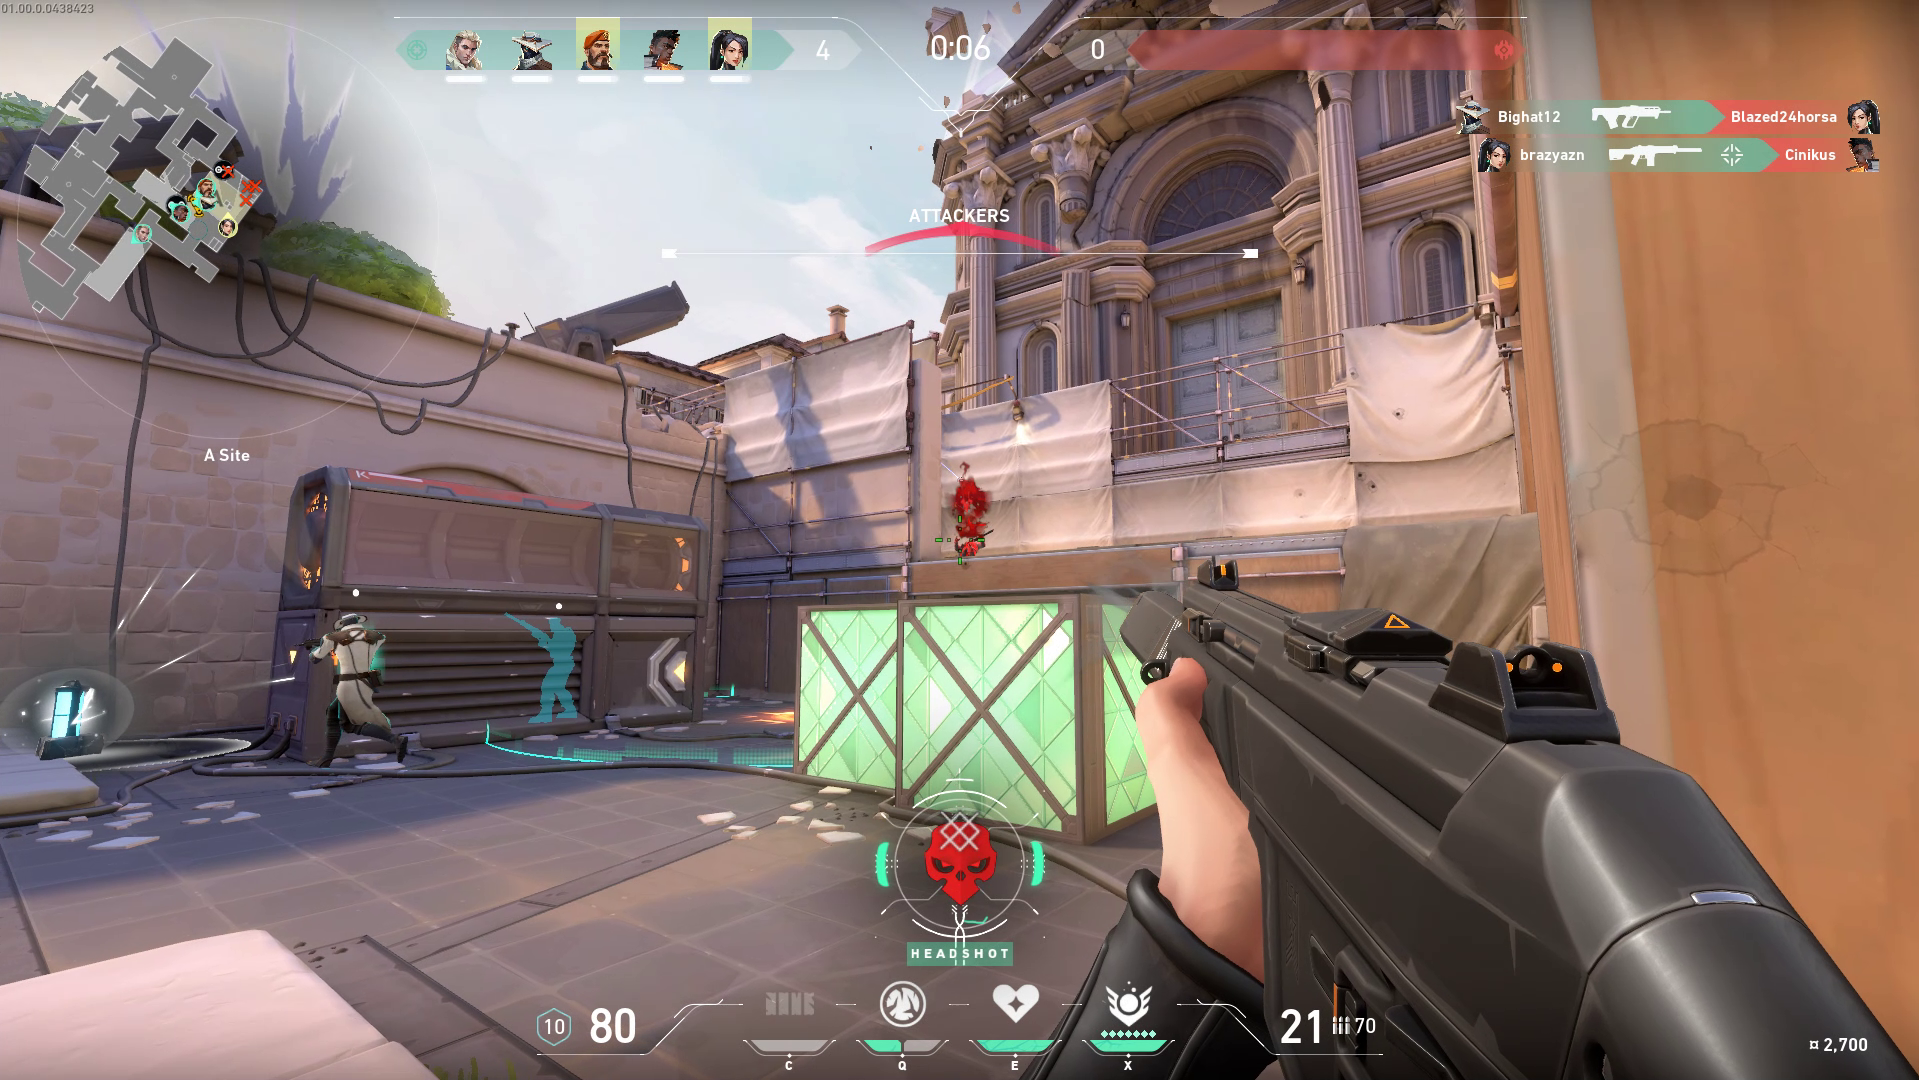
\includegraphics[width=\linewidth]{images/valorant_gameplay.png}
    \captionof*{figure}{Valorant - 120 FPS Gaming}
  \end{minipage}%
  \hfill
  \pause
  \begin{minipage}{0.45\textwidth}
    \centering
    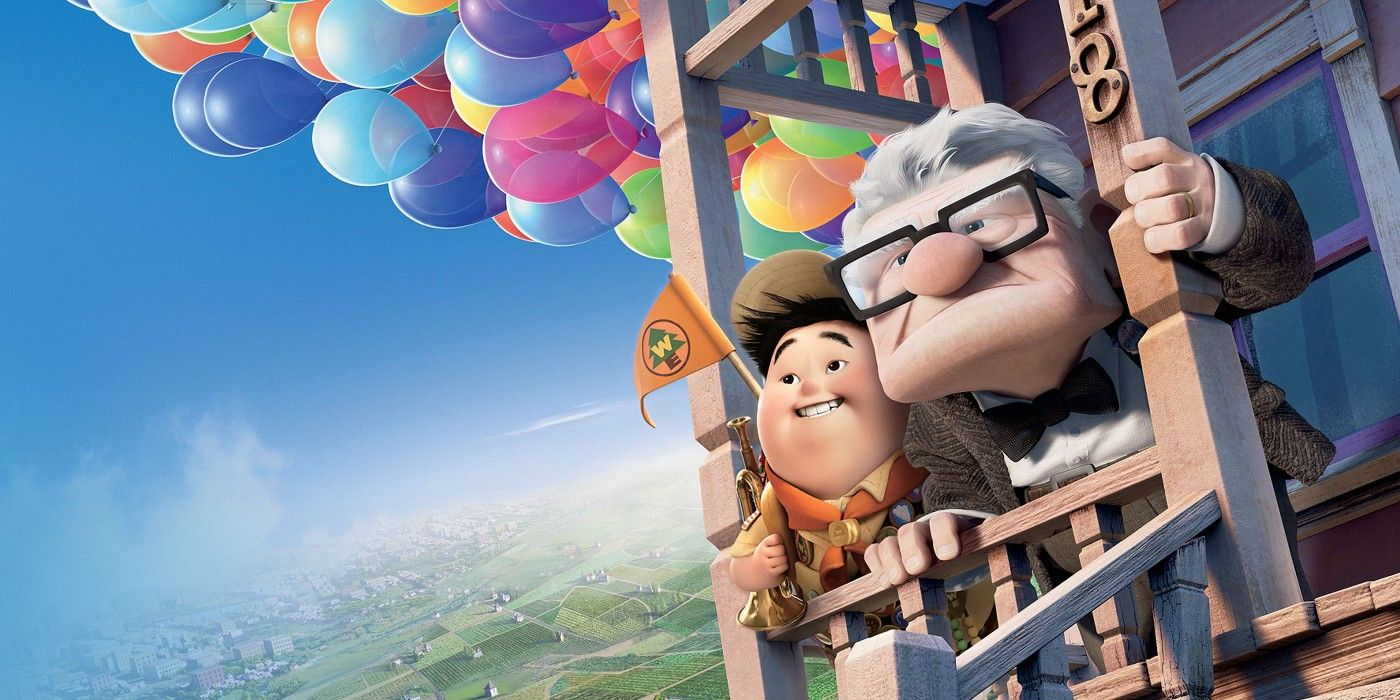
\includegraphics[width=\linewidth]{images/pixar_movie.jpg}
    \captionof*{figure}{Pixar Movie - 30 hours per frame}
  \end{minipage}

  \begin{itemize}
    \item<3-> \textbf{Real-time constraint:} Games need 60-120 FPS
    \item<4-> \textbf{Interactive experience:} User input must feel responsive
    \item<5-> \textbf{Trade-off:} Sacrifice physical accuracy for speed
    \item<6-> \textbf{Goal:} Images that look good enough, delivered fast enough
  \end{itemize}
\end{frame}

\section{The Speed vs Accuracy Trade-off}

\begin{frame}{Rasterization vs Ray Tracing: The Fundamental Choice}
  \begin{center}
    \begin{tikzpicture}[scale=0.9]
      % Rasterization side
      \node[rectangle, draw, minimum width=3cm, minimum height=2cm, fill=PrimaryColor!20] (raster) at (0,0) {\faIcon{tachometer-alt} Rasterization};
      \node[above] at (0,1.5) {\textbf{Fast Approximations}};

      % Ray tracing side
      \node[rectangle, draw, minimum width=3cm, minimum height=2cm, fill=AccentColor!20] (ray) at (6,0) {\faIcon{eye} Ray Tracing};
      \node[above] at (6,1.5) {\textbf{Physical Accuracy}};

      % Trade-off arrow
      \draw[<->, very thick, SecondaryColor]
      (raster.east) -- (ray.west)
      node[midway, above, text=SecondaryColor, font=\footnotesize]{Trade-off};

      % Characteristics
      \node[below] at (0,-2.5) {
        \begin{minipage}{4cm}
          \textcolor{PrimaryColor}{\textbf{Rasterization:}}
          \begin{itemize}
              \scriptsize
            \item 60-240 FPS
            \item Clever approximations
            \item Hardware optimized
            \item "Good enough" quality
          \end{itemize}
        \end{minipage}
      };

      \node[below] at (6,-2.5) {
        \begin{minipage}{4cm}
          \textcolor{AccentColor}{\textbf{Ray Tracing:}}
          \begin{itemize}
              \scriptsize
            \item 0.1-30 FPS
            \item Physical simulation
            \item Computationally heavy
            \item Photorealistic
          \end{itemize}
        \end{minipage}
      };
    \end{tikzpicture}
  \end{center}
\end{frame}

\begin{frame}{The Real-Time Graphics Challenge}
  \begin{columns}
    \begin{column}{0.6\textwidth}
      \begin{conceptbox}{Time Budget at 60 FPS}
        \begin{center}
          \large $\frac{1}{60} = 16.67$ milliseconds per frame
        \end{center}

        \vspace{0.3cm}
        \textbf{What needs to happen:}
        \begin{itemize}
          \item Process input
          \item Update game logic
          \item Render graphics
          \item Present to screen
        \end{itemize}

        \vspace{0.3cm}
        \textbf{Graphics budget:} $\sim$10-12ms
      \end{conceptbox}
    \end{column}
    \begin{column}{0.4\textwidth}
      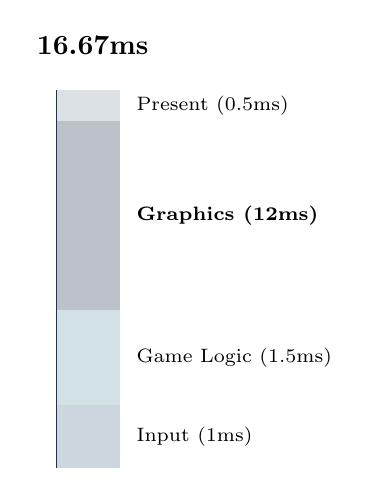
\begin{tikzpicture}[scale=0.8]
        % Timeline
        \draw[thick, PrimaryColor] (0,0) -- (0,6);
        \node[left] at (1.6,6.7) {\textbf{16.67ms}};

        % Segments
        \fill[SecondaryColor!30] (0,0) rectangle (1,1);
        \node[right] at (1.1,0.5) {\scriptsize Input (1ms)};

        \fill[AccentColor!30] (0,1) rectangle (1,2.5);
        \node[right] at (1.1,1.75) {\scriptsize Game Logic (1.5ms)};

        \fill[PrimaryColor!30] (0,2.5) rectangle (1,5.5);
        \node[right] at (1.1,4) {\scriptsize \textbf{Graphics (12ms)}};

        \fill[LightGray] (0,5.5) rectangle (1,6);
        \node[right] at (1.1,5.75) {\scriptsize Present (0.5ms)};

      \end{tikzpicture}
    \end{column}
  \end{columns}
\end{frame}

\begin{frame}{How Rasterization Achieves Speed}
  \begin{center}
    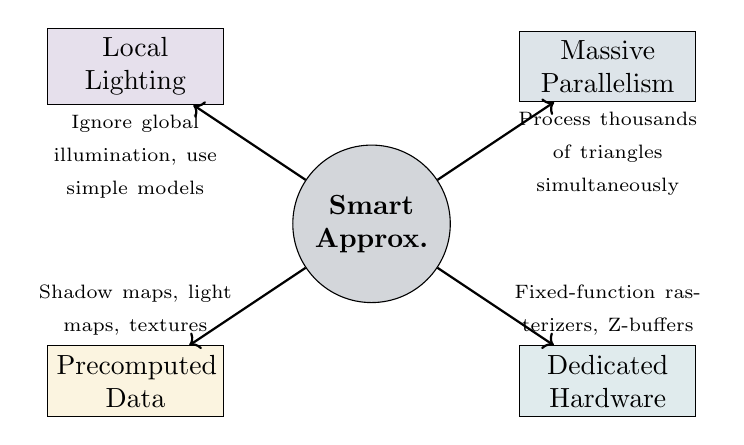
\begin{tikzpicture}[scale=1]
      % Central concept
      \node[circle, draw, fill=PrimaryColor!20, minimum size=2cm] (center) at (0,0) {
        \begin{minipage}{1.5cm}
          \centering
          \textbf{Smart} \\
          \textbf{Approx.}
        \end{minipage}
      };

      % Surrounding strategies
      \node[rectangle, draw, fill=SecondaryColor!20, text width=2cm, text centered] (parallel) at (3,2) {
        Massive \\
        Parallelism
      };

      \node[rectangle, draw, fill=AccentColor!20, text width=2cm, text centered] (hardware) at (3,-2) {
        Dedicated \\
        Hardware
      };

      \node[rectangle, draw, fill=ObjectColor!20, text width=2cm, text centered] (approx) at (-3,2) {
        Local \\
        Lighting
      };

      \node[rectangle, draw, fill=LightColor!20, text width=2cm, text centered] (cached) at (-3,-2) {
        Precomputed \\
        Data
      };

      % Connections
      \draw[->, thick] (center) -- (parallel);
      \draw[->, thick] (center) -- (hardware);
      \draw[->, thick] (center) -- (approx);
      \draw[->, thick] (center) -- (cached);

      % Examples
      \node[below, text width=2.5cm, text centered] at (parallel.south) {
        \scriptsize Process thousands of triangles simultaneously
      };

      \node[above, text width=2.5cm, text centered] at (hardware.north) {
        \scriptsize Fixed-function rasterizers, Z-buffers
      };

      \node[below, text width=2.5cm, text centered] at (approx.south) {
        \scriptsize Ignore global illumination, use simple models
      };

      \node[above, text width=2.5cm, text centered] at (cached.north) {
        \scriptsize Shadow maps, light maps, textures
      };
    \end{tikzpicture}
  \end{center}
\end{frame}

\begin{frame}{The Clever Approximations}
  \begin{columns}
    \begin{column}{0.5\textwidth}
      \begin{raybox}{What We Skip}
        \begin{itemize}
          \item \textbf{Global illumination:} No light bouncing
          \item \textbf{Perfect shadows:} Use shadow maps
          \item \textbf{Perfect reflections:} Use environment maps
          \item \textbf{Complex materials:} Simplified BRDFs
        \end{itemize}
      \end{raybox}
    \end{column}
    \begin{column}{0.5\textwidth}
      \begin{conceptbox}{What We Gain}
        \begin{itemize}
          \item \textbf{Predictable performance:} Linear with triangle count
          \item \textbf{Hardware optimization:} Purpose-built silicon
          \item \textbf{Real-time interaction:} Immediate feedback
          \item \textbf{Scalable quality:} Adjust for performance
        \end{itemize}
      \end{conceptbox}
    \end{column}
  \end{columns}

\end{frame}

\section{Ray Generation}




\begin{frame}{Ray Generation Mathematics}
    \begin{columns}
        \begin{column}{0.5\textwidth}
            \begin{tikzpicture}[scale=0.7]
                % Define 3D styles for math diagram
                \tikzset{
                    camera/.style={fill=PrimaryColor!60, draw=PrimaryColor!80, rectangle, minimum size=8pt},
                    image plane/.style={fill=AccentColor!10, draw=AccentColor!50, opacity=0.8}
                }

                % Camera position
                \node[camera] (camera) at (0,0,0) {\faIcon{camera}};
                \node[below] at (0,-0.6,0) {\small $\mathbf{e}$};

                % Image plane with mathematical annotations
                \begin{scope}[canvas is zy plane at x=2.5]
                    \fill[image plane] (-1.5,-1.5) rectangle (1.5,1.5);

                    % Sample pixel
                    \fill[AccentColor!80] (0.5,0.8) rectangle (0.8,1.1);
                    \fill[red!70] (0.65, 0.95) circle (0.05);

                    % Dimensions
                    \draw[<->, thin] (-1.5,-1.8) -- (1.5,-1.8);
                    \node[below] at (0,-1.8) {\small $n_x$};
                    \draw[<->, thin] (-1.8,-1.5) -- (-1.8,1.5);
                    \node[left] at (-1.8,0) {\small $n_y$};

                    % Pixel coordinates
                    \draw[dashed, thin] (0.5,0.8) -- (0.5,-1.8);
                    \draw[dashed, thin] (-1.8,0.8) -- (0.5,0.8);
                    \node[below] at (0.5,-1.6) {\tiny $i$};
                    \node[left] at (-1.6,0.8) {\tiny $j$};
                \end{scope}

                % Ray from camera through pixel
                \draw[ray, very thick] (camera) -- (0.65, 0.95);
                \draw[ray, dashed, thick] (0.65, 0.95) -- (4, 1.5, 1.5);

                % Distance annotation
                \draw[<->, thin] (0,0.3,0) -- (2.5,0.3,0);
                \node[above] at (1.25,0.3,0) {\small $d$};

                % Coordinate system
                \draw[<->, thick, PrimaryColor] (0,0,0) -- (1,0,0);
                \draw[<->, thick, PrimaryColor] (0,0,0) -- (0,1,0);
                \draw[<->, thick, PrimaryColor] (0,0,0) -- (0,0,1);
                \node[below right] at (1,0,0) {\small $\mathbf{u}$};
                \node[above] at (0,1,0) {\small $\mathbf{v}$};
                \node[below] at (0,0,1) {\small $\mathbf{w}$};
            \end{tikzpicture}
        \end{column}
        \begin{column}{0.5\textwidth}
            \begin{mathbox}{Ray Equation}
                For pixel $(i,j)$:
                \begin{align}
                    s & = \frac{i + 0.5}{n_x} \\
                    t & = \frac{j + 0.5}{n_y}
                \end{align}

                \vspace{0.2cm}
                \textbf{Ray direction:}
                \begin{align}
                    \mathbf{d} & = (s - 0.5) \cdot \text{FOV} \cdot \mathbf{u}       \\
                               & \quad + (t - 0.5) \cdot \text{FOV} \cdot \mathbf{v} \\
                               & \quad + d \cdot \mathbf{w}
                \end{align}

                \vspace{0.2cm}
                \textbf{Parametric ray:}
                \begin{equation}
                    \mathbf{r}(\lambda) = \mathbf{e} + \lambda \mathbf{d}
                \end{equation}
            \end{mathbox}

            \vspace{0.3cm}
            \begin{itemize}
                \item $\mathbf{e}$: camera position
                \item $\{\mathbf{u}, \mathbf{v}, \mathbf{w}\}$: orthonormal basis
                \item $d$: distance to image plane
                \item FOV: field of view factor
                \item $\lambda \geq 0$: ray parameter
            \end{itemize}
        \end{column}
    \end{columns}
\end{frame}
% \section{Rays and Cameras}

\begin{frame}{The Pinhole Camera Model}
    \begin{columns}
        \begin{column}{0.5\textwidth}
            \begin{mathbox}{Pinhole Camera}
                \textbf{Key Properties:}
                \begin{itemize}
                    \item Point aperture (no lens)
                    \item Perfect focus everywhere
                    \item Linear perspective
                    \item No depth of field
                \end{itemize}

                \vspace{0.3cm}
                \textbf{Ray Generation:}
                \begin{align}
                    \mathbf{R_o} & = \mathbf{eye}                  \\
                    \mathbf{R_d} & = \mathbf{pixel} - \mathbf{eye}
                \end{align}
            \end{mathbox}
        \end{column}
        \begin{column}{0.5\textwidth}
            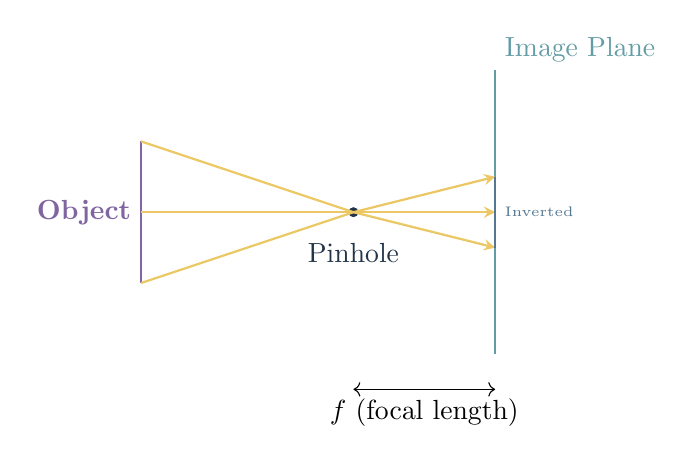
\begin{tikzpicture}[scale=0.9]
                % Pinhole
                \fill[PrimaryColor] (0,0) circle (2pt);
                \node[below] at (0,-0.3) {\textcolor{PrimaryColor}{Pinhole}};

                % Image plane
                \draw[thick, AccentColor] (2,-2) -- (2,2);
                \node[right] at (2,2.3) {\textcolor{AccentColor}{Image Plane}};

                % Object
                \draw[thick, ObjectColor] (-3,1) -- (-3,-1);
                \node[left] at (-3,0) {\objectcolor{Object}};

                % Light rays
                \draw[lightray] (-3,1) -- (0,0) -- (2,-0.5);
                \draw[lightray] (-3,0) -- (0,0) -- (2,0);
                \draw[lightray] (-3,-1) -- (0,0) -- (2,0.5);

                % Projected image
                \draw[thick, SecondaryColor] (2,-0.5) -- (2,0.5);
                \node[right] at (2,0) {\textcolor{SecondaryColor}{\tiny Inverted}};

                % Focal length
                \draw[<->, thin] (0,-2.5) -- (2,-2.5);
                \node[below] at (1,-2.5) {$f$ (focal length)};
            \end{tikzpicture}
        \end{column}
    \end{columns}

    \begin{conceptbox}{Physical Reality}
        Real pinhole cameras exist! They create sharp images but require long exposure times due to tiny aperture.
    \end{conceptbox}
\end{frame}

\begin{frame}{Simplified Pinhole Camera}
    \begin{columns}
        \begin{column}{0.5\textwidth}
            \begin{mathbox}{Simplification}
                \textbf{Problem:} Real pinhole creates inverted image

                \textbf{Solution:} Place image plane in front!
                \begin{align}
                    \mathbf{pixel} & = \mathbf{eye} + d \cdot \mathbf{w} + u \cdot \mathbf{u} + v \cdot \mathbf{v}
                \end{align}

                where:
                \begin{itemize}
                    \item $d$ = distance to image plane
                    \item $u, v$ = pixel coordinates
                    \item $\mathbf{u}, \mathbf{v}, \mathbf{w}$ = camera basis
                \end{itemize}
            \end{mathbox}
        \end{column}
        \begin{column}{0.5\textwidth}
            \begin{tikzpicture}[scale=0.9]
                % Eye/Camera
                \node[eye] (eye) at (0,0) {\faIcon{eye}};
                \node[below] at (0,-0.5) {\textcolor{PrimaryColor}{Eye}};

                % Image plane (in front)
                \draw[thick, AccentColor] (2,-2) -- (2,2);
                \node[right] at (2,2.3) {\textcolor{AccentColor}{Image Plane}};

                % Pixel grid
                \foreach \y in {-1.5,-1,-0.5,0,0.5,1,1.5} {
                        \draw[thin, gray] (1.8,\y) -- (2.2,\y);
                    }

                % Object
                \draw[thick, ObjectColor] (4,1.5) -- (4,-1.5);
                \node[right] at (4,0) {\objectcolor{Object}};

                % Rays through pixels
                \draw[ray] (eye) -- (2,1.5) -- (4,1.5);
                \draw[ray] (eye) -- (2,0) -- (4,0);
                \draw[ray] (eye) -- (2,-1.5) -- (4,-1.5);

                % Coordinate system
                \draw[->, thin] (0,2.5) -- (0,0) -- (2.5,0);
                \node[left] at (0,1.25) {$\mathbf{v}$};
                \node[below] at (1.25,0) {$\mathbf{u}$};
                \node[above right] at (1.5,1.5) {$\mathbf{w}$};

                % Distance
                \draw[<->, thin] (0,-2.5) -- (2,-2.5);
                \node[below] at (1,-2.5) {$d$};
            \end{tikzpicture}
        \end{column}
    \end{columns}

    \begin{conceptbox}{Advantage}
        \textbf{Upright image}, easier ray generation, same perspective as real pinhole!
    \end{conceptbox}
\end{frame}

\begin{frame}{Orthographic Camera}
    \begin{columns}
        \begin{column}{0.5\textwidth}
            \begin{mathbox}{Orthographic Projection}
                \textbf{Key Properties:}
                \begin{itemize}
                    \item No perspective distortion
                    \item Parallel projection rays
                    \item Objects same size regardless of distance
                    \item Infinite focal length
                \end{itemize}

                \textbf{Ray Generation:}
                \begin{align}
                    \mathbf{R_o} & = \mathbf{pixel}                \\
                    \mathbf{R_d} & = \mathbf{w} \text{ (constant)}
                \end{align}
            \end{mathbox}
        \end{column}
        \begin{column}{0.5\textwidth}
            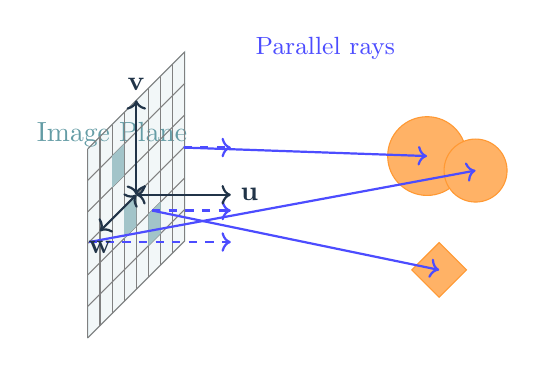
\begin{tikzpicture}[scale=0.8]
                % Define 3D styles for orthographic
                \tikzset{
                    ortho plane/.style={fill=AccentColor!10, draw=AccentColor!50, opacity=0.8},
                    ortho pixel/.style={fill=AccentColor!60, thick},
                    ortho ray/.style={->, thick, blue!70},
                    ortho object/.style={fill=orange!60, draw=orange!80}
                }

                % Image plane in 3D (using canvas is plane)
                \begin{scope}[canvas is zy plane at x=0]
                    % Background image plane
                    \fill[ortho plane] (-2,-1.5) rectangle (2,1.5);
                    \node[left] at (-2.5,0) {\textcolor{AccentColor}{Image Plane}};

                    % Pixel grid
                    \foreach \y in {-1.5,-1,-0.5,0,0.5,1,1.5} {
                            \draw[thin, gray] (-2,\y) -- (2,\y);
                        }
                    \foreach \z in {-2,-1.5,-1,-0.5,0,0.5,1,1.5,2} {
                            \draw[thin, gray] (\z,-1.5) -- (\z,1.5);
                        }

                    % Sample pixels
                    \fill[ortho pixel] (0.5,0.5) rectangle (1,1);
                    \fill[ortho pixel] (-1,-1) rectangle (-0.5,-0.5);
                    \fill[ortho pixel] (0,-0.5) rectangle (0.5,0);
                \end{scope}

                % Objects in 3D scene
                \node[ortho object, circle, minimum size=1cm] (sphere1) at (5,1,1) {};
                \node[ortho object, circle, minimum size=0.8cm] (sphere2) at (5,0,-1) {};
                \node[ortho object, diamond, minimum size=0.7cm] (diamond) at (5,-1,0.5) {};

                % Parallel rays from pixels (orthographic property)
                \draw[ortho ray] (0.75,0.75,0) -- (5,1,1);
                \draw[ortho ray] (-0.75,-0.75,0) -- (5,0,-1);
                \draw[ortho ray] (0.25,-0.25,0) -- (5,-1,0.5);

                % All rays parallel to w direction
                \draw[ortho ray, dashed] (0.75,0.75,0) -- (1.5,0.75,0);
                \draw[ortho ray, dashed] (-0.75,-0.75,0) -- (1.5,-0.75,0);
                \draw[ortho ray, dashed] (0.25,-0.25,0) -- (1.5,-0.25,0);

                % 3D coordinate system
                \draw[<->, thick, PrimaryColor] (0,0,0) -- (1.5,0,0);
                \draw[<->, thick, PrimaryColor] (0,0,0) -- (0,1.5,0);
                \draw[<->, thick, PrimaryColor] (0,0,0) -- (0,0,1.5);
                \node[right] at (1.5,0,0) {\textcolor{PrimaryColor}{$\mathbf{u}$}};
                \node[above] at (0,1.5,0) {\textcolor{PrimaryColor}{$\mathbf{v}$}};
                \node[below] at (0,0,1.5) {\textcolor{PrimaryColor}{$\mathbf{w}$}};

                % Label showing parallel rays
                \node[above] at (3,2,0) {\textcolor{blue!70}{\small Parallel rays}};
            \end{tikzpicture}
        \end{column}
    \end{columns}

    \begin{conceptbox}{Applications}
        \textbf{Technical drawings}, \textbf{CAD software}, \textbf{2D games}, architectural visualization
    \end{conceptbox}
\end{frame}

\begin{frame}{Perspective vs Orthographic}
    \begin{center}
        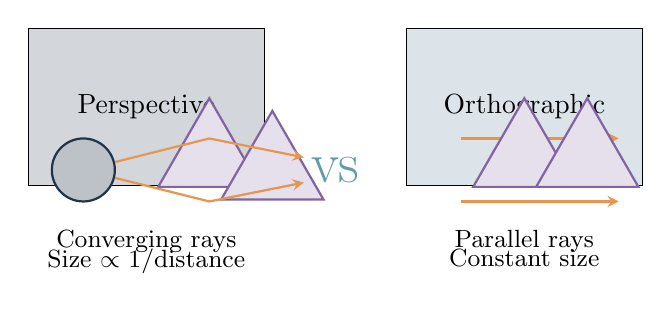
\begin{tikzpicture}[scale=0.8]
            % Perspective
            \node[rectangle, draw, minimum width=3cm, minimum height=2cm, fill=PrimaryColor!20] at (-3,2) {Perspective};
            \node[eye] (eye1) at (-4,1) {};
            \node[triangle] (near1) at (-2,1.2) {};
            \node[triangle] (far1) at (-1,1) {};
            \draw[ray] (eye1) -- (-2,1.5) -- (-0.5,1.2);
            \draw[ray] (eye1) -- (-2,0.5) -- (-0.5,0.8);
            \node[below] at (-3,0.2) {\small Converging rays};
            \node[below] at (-3,-0.1) {\small Size $\propto$ 1/distance};

            % vs
            \node at (0,1) {\huge \textcolor{AccentColor}{vs}};

            % Orthographic  
            \node[rectangle, draw, minimum width=3cm, minimum height=2cm, fill=SecondaryColor!20] at (3,2) {Orthographic};
            \draw[ray] (2,1.5) -- (4.5,1.5);
            \draw[ray] (2,0.5) -- (4.5,0.5);
            \node[triangle] (near2) at (3,1.2) {};
            \node[triangle] (far2) at (4,1.2) {};
            \node[below] at (3,0.2) {\small Parallel rays};
            \node[below] at (3,-0.1) {\small Constant size};
        \end{tikzpicture}
    \end{center}

    \vspace{0.5cm}
    \begin{columns}
        \begin{column}{0.5\textwidth}
            \begin{raybox}{When to use Perspective}
                \begin{itemize}
                    \item Natural/realistic scenes
                    \item Human vision simulation
                    \item Games and films
                    \item Depth perception important
                \end{itemize}
            \end{raybox}
        \end{column}
        \begin{column}{0.5\textwidth}
            \begin{raybox}{When to use Orthographic}
                \begin{itemize}
                    \item Technical illustrations
                    \item CAD/Engineering
                    \item UI elements overlay
                    \item Precise measurements
                \end{itemize}
            \end{raybox}
        \end{column}
    \end{columns}
\end{frame}

\begin{frame}{Thin Lens Camera: Fundamentals}
    \begin{columns}
        \begin{column}{0.5\textwidth}
            \begin{mathbox}{Gaussian Lens Equation}
                \textbf{Fundamental relationship:}
                \begin{align}
                    \frac{1}{f} = \frac{1}{z} + \frac{1}{z'}
                \end{align}

                \textbf{Where:}
                \begin{itemize}
                    \item $f$ = focal length of lens
                    \item $z$ = object distance from lens
                    \item $z'$ = image distance from lens
                \end{itemize}

                \vspace{0.3cm}
                \textbf{Key Properties:}
                \begin{itemize}
                    \item Objects at focal plane are in perfect focus
                    \item Other distances create blur (circle of confusion)
                    \item Aperture size controls depth of field
                \end{itemize}
            \end{mathbox}
        \end{column}
        \begin{column}{0.5\textwidth}
            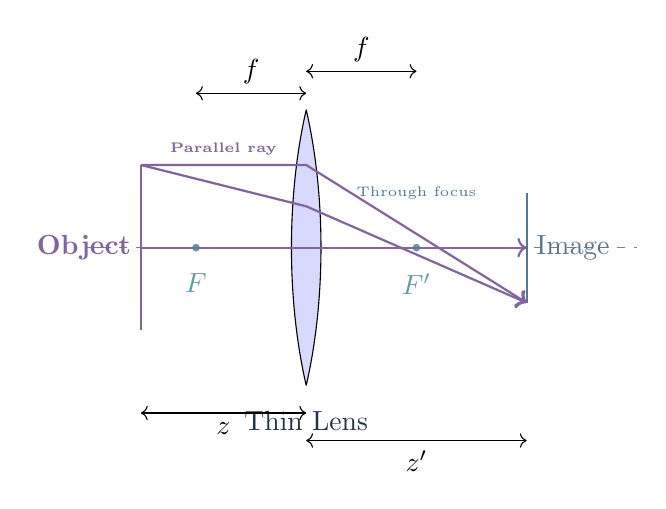
\begin{tikzpicture}[scale=0.7]
                % Define styles for thin lens
                % Optical axis
                \draw[optical axis] (-4,0) -- (6,0);
                
                % Thin lens at origin
                \lens{(0,0)}{2cm}{5cm};
                \node[below] at (0,-2.8) {\textcolor{PrimaryColor}{Thin Lens}};
                
                % Object at distance z
                \draw[thick, ObjectColor] (-3,-1.5) -- (-3,1.5);
                \node[left] at (-3,0) {\objectcolor{Object}};
                \draw[<->, thin] (-3,-3) -- (0,-3);
                \node[below] at (-1.5,-3) {$z$};
                
                % Image at distance z'
                \draw[thick, SecondaryColor] (4,-1) -- (4,1);
                \node[right] at (4,0) {\textcolor{SecondaryColor}{Image}};
                \draw[<->, thin] (0,-3.5) -- (4,-3.5);
                \node[below] at (2,-3.5) {$z'$};
                
                % Focal points
                \fill[AccentColor] (-2,0) circle (2pt);
                \fill[AccentColor] (2,0) circle (2pt);
                \node[below] at (-2,-0.3) {\textcolor{AccentColor}{$F$}};
                \node[below] at (2,-0.3) {\textcolor{AccentColor}{$F'$}};
                
                % Focal length markers
                \draw[<->, thin] (-2,2.8) -- (0,2.8);
                \node[above] at (-1,2.8) {$f$};
                \draw[<->, thin] (0,3.2) -- (2,3.2);
                \node[above] at (1,3.2) {$f$};
                
                % Principal rays
                \draw[object ray] (-3,1.5) -- (0,1.5) -- (4,-1);
                \draw[object ray] (-3,1.5) -- (0,0.75) -- (4,-1);
                \draw[object ray] (-3,0) -- (0,0) -- (4,0);
                
                % Ray labels
                \node[above] at (-1.5,1.5) {\objectcolor{\tiny Parallel ray}};
                \node[above] at (2,0.7) {\textcolor{SecondaryColor}{\tiny Through focus}};
            \end{tikzpicture}
        \end{column}
    \end{columns}

    \begin{conceptbox}{Real Camera Behavior}
        Unlike pinhole cameras, thin lens cameras exhibit \textbf{depth of field} - only objects at the focal distance are perfectly sharp.
    \end{conceptbox}
\end{frame}

\begin{frame}{Depth of Field and Circle of Confusion}
    \begin{columns}
        \begin{column}{0.5\textwidth}
            \begin{mathbox}{Circle of Confusion}
                \textbf{For objects not at focal distance:}
                \begin{align}
                    c = \frac{A}{z'} \left| z'_{focus} - z' \right|
                \end{align}

                \textbf{Where:}
                \begin{itemize}
                    \item $c$ = circle of confusion diameter
                    \item $A$ = aperture diameter
                    \item $z'$ = image distance for object
                    \item $z'_{focus}$ = image distance for focus
                \end{itemize}

                \vspace{0.3cm}
                \textbf{Depth of Field:}
                \begin{itemize}
                    \item Region where $c < $ acceptable limit
                    \item Larger aperture $\rightarrow$ shallower DOF
                    \item Smaller aperture $\rightarrow$ deeper DOF
                \end{itemize}
            \end{mathbox}
        \end{column}
        \begin{column}{0.5\textwidth}
            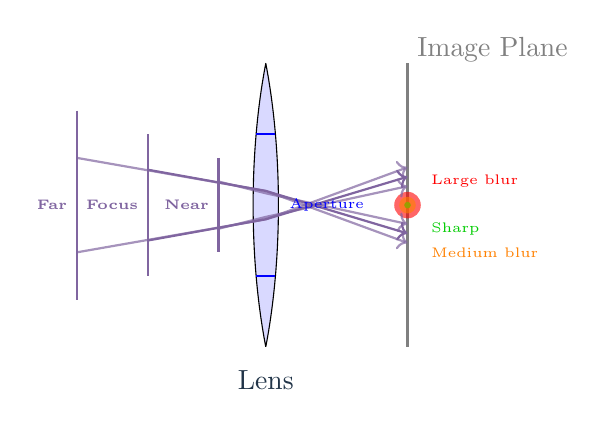
\begin{tikzpicture}[scale=0.6]
                % Three object planes at different distances
                \draw[thick, ObjectColor] (-4,2) -- (-4,-2);
                \draw[thick, ObjectColor] (-2.5,1.5) -- (-2.5,-1.5);
                \draw[thick, ObjectColor] (-1,1) -- (-1,-1);
                
                \node[left] at (-4,0) {\objectcolor{\tiny Far}};
                \node[left] at (-2.5,0) {\objectcolor{\tiny Focus}};
                \node[left] at (-1,0) {\objectcolor{\tiny Near}};
                
                % Lens
                \lens{(0,0)}{2cm}{6cm};
                \node[below] at (0,-3.3) {\textcolor{PrimaryColor}{Lens}};
                
                % Image plane
                \draw[thick, gray] (3,-3) -- (3,3);
                \node[right] at (3,3.3) {\textcolor{gray}{Image Plane}};
                
                % Rays from far object (out of focus)
                \draw[object ray, opacity=0.7] (-4,1) -- (0,0.3) -- (3,-0.8);
                \draw[object ray, opacity=0.7] (-4,-1) -- (0,-0.3) -- (3,0.8);
                \fill[red, opacity=0.6] (3,0) circle (8pt);
                \node[right] at (3.3,0.5) {\textcolor{red}{\tiny Large blur}};
                
                % Rays from focus object (sharp)
                \draw[object ray] (-2.5,0.75) -- (0,0.3) -- (3,-0.6);
                \draw[object ray] (-2.5,-0.75) -- (0,-0.3) -- (3,0.6);
                \fill[green!80!black] (3,0) circle (2pt);
                \node[right] at (3.3,-0.5) {\textcolor{green!80!black}{\tiny Sharp}};
                
                % Rays from near object (out of focus)
                \draw[object ray, opacity=0.7] (-1,0.5) -- (0,0.25) -- (3,-0.4);
                \draw[object ray, opacity=0.7] (-1,-0.5) -- (0,-0.25) -- (3,0.4);
                \fill[orange, opacity=0.6] (3,0) circle (5pt);
                \node[right] at (3.3,-1) {\textcolor{orange}{\tiny Medium blur}};
                
                % Aperture indication
                \draw[thick, blue] (-0.2,-1.5) -- (0.2,-1.5);
                \draw[thick, blue] (-0.2,1.5) -- (0.2,1.5);
                \node[right] at (0.3,0) {\textcolor{blue}{\tiny Aperture}};
            \end{tikzpicture}
        \end{column}
    \end{columns}

    \begin{conceptbox}{Artistic Control}
        \textbf{Shallow DOF}: Subject isolation, portrait photography\\
        \textbf{Deep DOF}: Landscape photography, technical documentation
    \end{conceptbox}
\end{frame}

\begin{frame}{Aperture Effects on Depth of Field}
    \begin{center}
        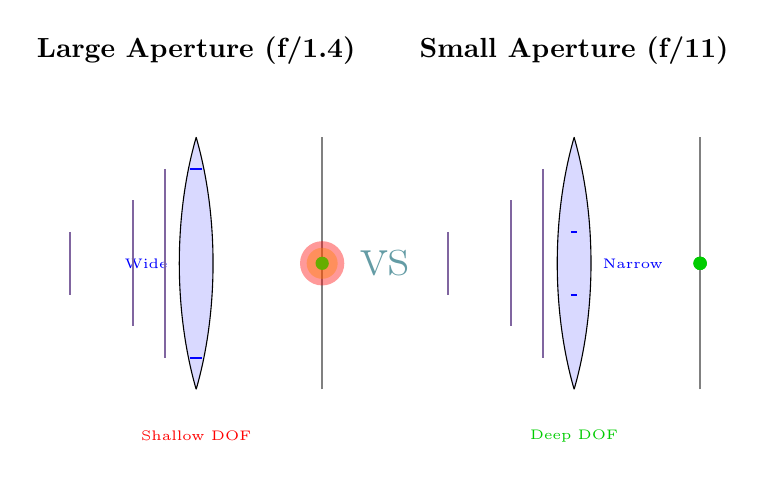
\begin{tikzpicture}[scale=0.8]
            % Large aperture scene
            \node[above] at (-3,3) {\textbf{Large Aperture (f/1.4)}};
            
            % Lens with large aperture
            \lens{(-3,0)}{2cm}{4cm};
            \draw[thick, blue] (-3.1,-1.5) -- (-2.9,-1.5);
            \draw[thick, blue] (-3.1,1.5) -- (-2.9,1.5);
            \node[left] at (-3.3,0) {\textcolor{blue}{\tiny Wide}};
            
            % Objects at different distances
            \draw[thick, ObjectColor] (-5,0.5) -- (-5,-0.5);
            \draw[thick, ObjectColor] (-4,1) -- (-4,-1);
            \draw[thick, ObjectColor] (-3.5,1.5) -- (-3.5,-1.5);
            
            % Image plane
            \draw[thick, gray] (-1,-2) -- (-1,2);
            
            % Blur circles (large aperture = shallow DOF)
            \fill[red, opacity=0.4] (-1,0) circle (10pt);
            \fill[green!80!black] (-1,0) circle (3pt);
            \fill[orange, opacity=0.4] (-1,0) circle (7pt);
            
            \node[below] at (-3,-2.5) {\textcolor{red}{\tiny Shallow DOF}};
            
            % vs divider
            \node at (0,0) {\huge \textcolor{AccentColor}{vs}};
            
            % Small aperture scene
            \node[above] at (3,3) {\textbf{Small Aperture (f/11)}};
            
            % Lens with small aperture
            \lens{(3,0)}{2cm}{4cm};
            \draw[thick, blue] (2.95,-0.5) -- (3.05,-0.5);
            \draw[thick, blue] (2.95,0.5) -- (3.05,0.5);
            \node[right] at (3.3,0) {\textcolor{blue}{\tiny Narrow}};
            
            % Objects at different distances
            \draw[thick, ObjectColor] (1,0.5) -- (1,-0.5);
            \draw[thick, ObjectColor] (2,1) -- (2,-1);
            \draw[thick, ObjectColor] (2.5,1.5) -- (2.5,-1.5);
            
            % Image plane
            \draw[thick, gray] (5,-2) -- (5,2);
            
            % Blur circles (small aperture = deep DOF)
            \fill[green!80!black] (5,0) circle (3pt);
            \fill[green!80!black] (5,0) circle (3pt);
            \fill[green!80!black] (5,0) circle (3pt);
            
            \node[below] at (3,-2.5) {\textcolor{green!80!black}{\tiny Deep DOF}};
        \end{tikzpicture}
    \end{center}

    \vspace{0.5cm}
    \begin{columns}
        \begin{column}{0.5\textwidth}
            \begin{raybox}{Large Aperture}
                \begin{itemize}
                    \item More light gathering
                    \item Faster shutter speeds
                    \item Shallow depth of field
                    \item Background blur (bokeh)
                \end{itemize}
            \end{raybox}
        \end{column}
        \begin{column}{0.5\textwidth}
            \begin{raybox}{Small Aperture}
                \begin{itemize}
                    \item Less light gathering
                    \item Slower shutter speeds
                    \item Deep depth of field
                    \item Everything in focus
                \end{itemize}
            \end{raybox}
        \end{column}
    \end{columns}
\end{frame}

\begin{frame}{Thin Lens Ray Generation}
    \begin{columns}
        \begin{column}{0.5\textwidth}
            \begin{mathbox}{Ray Sampling Process}
                \textbf{1. Sample pixel position} $(x, y)$
                
                \textbf{2. Sample lens position:}
                \begin{align}
                    (u, v) &\sim \text{Uniform disk}\\
                    \mathbf{p}_{lens} &= (u \cdot r, v \cdot r, 0)
                \end{align}
                
                \textbf{3. Compute focal point:}
                \begin{align}
                    \mathbf{p}_{focus} &= \mathbf{p}_{pixel} \cdot \frac{f_{dist}}{n}
                \end{align}
                
                \textbf{4. Ray from lens to focal point:}
                \begin{align}
                    \mathbf{R_o} &= \mathbf{p}_{lens}\\
                    \mathbf{R_d} &= \mathbf{p}_{focus} - \mathbf{p}_{lens}
                \end{align}
                
                where $r$ = aperture radius, $f_{dist}$ = focus distance
            \end{mathbox}
        \end{column}
        \begin{column}{0.5\textwidth}
            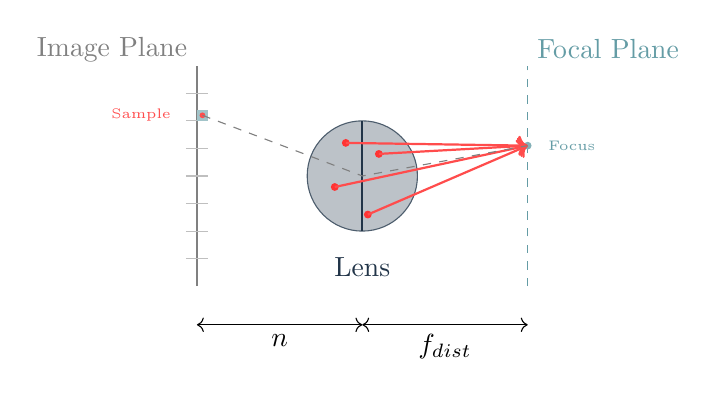
\begin{tikzpicture}[scale=0.7]
                % Define styles for ray generation
                \tikzset{
                    lens disk/.style={fill=PrimaryColor!30, draw=PrimaryColor!80},
                    sample point/.style={fill=red!80, circle, inner sep=1pt},
                    focal point/.style={fill=AccentColor!80, circle, inner sep=1.5pt},
                    sample ray/.style={->, thick, red!70},
                    focal plane/.style={dashed, AccentColor}
                }

                % Image plane
                \draw[thick, gray] (-3,-2) -- (-3,2);
                \node[left] at (-3,2.3) {\textcolor{gray}{Image Plane}};
                
                % Pixel grid
                \foreach \y in {-1.5,-1,-0.5,0,0.5,1,1.5} {
                        \draw[thin, gray!50] (-3.2,\y) -- (-2.8,\y);
                    }
                
                % Sample pixel
                \fill[AccentColor!60] (-3,1) rectangle (-2.8,1.2);
                \fill[red!70] (-2.9,1.1) circle (1.5pt);
                \node[left] at (-3.3,1.1) {\textcolor{red!70}{\tiny Sample}};
                
                % Lens disk
                \fill[lens disk] (0,0) circle (1);
                \draw[thick, PrimaryColor] (0,-1) -- (0,1);
                \node[below] at (0,-1.3) {\textcolor{PrimaryColor}{Lens}};
                
                % Sample points on lens
                \node[sample point] at (0.3,0.4) {};
                \node[sample point] at (-0.5,-0.2) {};
                \node[sample point] at (0.1,-0.7) {};
                \node[sample point] at (-0.3,0.6) {};
                
                % Focal plane
                \draw[focal plane] (3,-2) -- (3,2);
                \node[right] at (3,2.3) {\textcolor{AccentColor}{Focal Plane}};
                
                % Focal point (where pixel ray hits focal plane)
                \fill[focal point] (3,0.55) circle (2pt);
                \node[right] at (3.2,0.55) {\textcolor{AccentColor}{\tiny Focus}};
                
                % Sample rays from lens points to focal point
                \draw[sample ray] (0.3,0.4) -- (3,0.55);
                \draw[sample ray] (-0.5,-0.2) -- (3,0.55);
                \draw[sample ray] (0.1,-0.7) -- (3,0.55);
                \draw[sample ray] (-0.3,0.6) -- (3,0.55);
                
                % Central ray (through lens center)
                \draw[dashed, gray] (-2.9,1.1) -- (0,0) -- (3,0.55);
                
                % Distance markers
                \draw[<->, thin] (-3,-2.7) -- (0,-2.7);
                \node[below] at (-1.5,-2.7) {$n$};
                \draw[<->, thin] (0,-2.7) -- (3,-2.7);
                \node[below] at (1.5,-2.7) {$f_{dist}$};
            \end{tikzpicture}
        \end{column}
    \end{columns}

    \begin{conceptbox}{Monte Carlo Integration}
        Multiple samples per pixel with different lens positions create realistic \textbf{depth of field blur}
    \end{conceptbox}
\end{frame}



\begin{frame}{Other Camera Types}
    \begin{columns}
        \begin{column}{0.5\textwidth}
            \begin{conceptbox}{Fish-eye Camera}
                \begin{itemize}
                    \item Very wide field of view (>180°)
                    \item Non-linear distortion
                    \item Curved ray paths
                    \item Surveillance, VR applications
                \end{itemize}
            \end{conceptbox}

            \vspace{0.3cm}
            \begin{conceptbox}{Environment Camera}
                \begin{itemize}
                    \item 360° panoramic view
                    \item Spherical or cylindrical
                    \item HDRI environment maps
                    \item VR content creation
                \end{itemize}
            \end{conceptbox}
        \end{column}
        \begin{column}{0.5\textwidth}
            \begin{tikzpicture}[scale=0.8]
                % Fish-eye illustration
                \node[above] at (0,3) {\textbf{Fish-eye FOV}};
                \node[eye] (fisheye) at (0,2) {\faIcon{eye}};
                \draw[ray, bend left=30] (fisheye) to (2,3);
                \draw[ray] (fisheye) -- (2,2);
                \draw[ray, bend right=30] (fisheye) to (2,1);
                \draw[ray, bend left=60] (fisheye) to (1,3.5);
                \draw[ray, bend right=60] (fisheye) to (1,0.5);
                \node[right] at (2.2,2) {\tiny Wide FOV};

                % Motion blur illustration  
                \node[above] at (0,0.5) {\textbf{Motion Blur}};
                \draw[thick, gray] (-1,-1) -- (1,-1);
                \node[left] at (-1,-1) {\textcolor{gray}{\tiny Image plane}};
                \draw[ray, opacity=0.3] (-0.5,-0.5) -- (0.5,-1);
                \draw[ray, opacity=0.5] (-0.3,-0.5) -- (0.3,-1);
                \draw[ray, opacity=0.7] (-0.1,-0.5) -- (0.1,-1);
                \draw[ray] (0.1,-0.5) -- (-0.1,-1);
                \node[right] at (1.2,-1) {\tiny Multiple samples};
            \end{tikzpicture}
        \end{column}
    \end{columns}

    \begin{columns}
        \begin{column}{0.5\textwidth}
            \begin{conceptbox}{Environment Camera}
                \begin{itemize}
                    \item 360° panoramic view
                    \item Spherical or cylindrical
                    \item HDRI environment maps
                    \item VR content creation
                \end{itemize}
            \end{conceptbox}
        \end{column}
        \begin{column}{0.5\textwidth}
            \begin{conceptbox}{Motion Blur Camera}
                \begin{itemize}
                    \item Simulates camera/object motion
                    \item Multiple time samples
                    \item Temporal anti-aliasing
                    \item Dynamic scene rendering
                \end{itemize}
            \end{conceptbox}
        \end{column}
    \end{columns}
\end{frame}




\begin{frame}{Camera Representation}
    \begin{center}
        \begin{tikzpicture}[scale=0.7]
            % Define 3D styles
            \tikzset{
                camera/.style={fill=PrimaryColor!60, draw=PrimaryColor!80, rectangle, minimum size=8pt},
                image plane/.style={fill=AccentColor!10, draw=AccentColor!50, opacity=0.8},
                pixel/.style={fill=AccentColor!60, thick},
                primary ray/.style={->, very thick, red!90},
                object/.style={fill=orange!60, draw=orange!80, circle, minimum size=12pt}
            }

            % 3D coordinate system
            \draw[<->, thick, PrimaryColor] (0,0,0) -- (1.5,0,0);
            \draw[<->, thick, PrimaryColor] (0,0,0) -- (0,1.5,0);
            \draw[<->, thick, PrimaryColor] (0,0,0) -- (0,0,2);
            \node[right] at (1.5,0,0) {\textcolor{PrimaryColor}{$\mathbf{u}$}};
            \node[above] at (0,1.5,0) {\textcolor{PrimaryColor}{$\mathbf{v}$}};
            \node[below] at (0,0,2) {\textcolor{PrimaryColor}{$\mathbf{w}$}};

            % Camera/Eye position in 3D space
            \node[eye] (camera) at (0,0,0) {\faIcon{camera}};
            % \node[below] at (0.2,-0.5,0) {\textcolor{PrimaryColor}{Camera}};


            \draw[thick, gray] (camera) -- (4,2,2);
            \draw[thick, gray] (camera) -- (4,-2,2);
            \draw[thick, gray] (camera) -- (4,2,-2);
            \draw[thick, gray] (camera) -- (4,-2,-2);

            % Objects in 3D scene
            \node[sphere, minimum size=1cm] (sphere1) at (8,1,2) {};
            \node[sphere, minimum size=0.8cm] (sphere2) at (7,-1,-1) {};
            \node[triangle, minimum size=1cm] (tri) at (9,0.5,0) {};

            \draw[<->, thick, gray] (0, 2.5, 0) -- (4, 2.5, 0) node[midway, above] {\textcolor{gray}{$n$}};

            \node[below] at (0, -0.5, 0) {\textcolor{PrimaryColor!80}{$\mathbf{e}$}};

            \begin{scope}[
                    ->,
                    plane x={(0.8944,-0.4472, 0)},
                    plane y={(0,0,-1)},
                    canvas is plane,
                ]
                \fill[PrimaryColor!30, opacity=0.3] 
                    (0,0) 
                    -- (2,0)
                    arc[start angle=0, end angle=25, radius=2]
                    -- (0,0)
                    -- (2,0)
                    arc[start angle=0, end angle=-25, radius=2]
                -- cycle;
                \draw[->, thick, PrimaryColor] (2,0) arc[start angle=0, end angle=25, radius=2];
                \draw[->, thick, PrimaryColor] (2,0) arc[start angle=0, end angle=-25, radius=2];
                \node[below] at (2.2,0.3) {\textcolor{PrimaryColor}{$fov$}};
            \end{scope}


            % Image plane in 3D (using canvas is plane)
            \begin{scope}[canvas is zy plane at x=4]
                % Background image plane
                \fill[image plane] (-2,-2) rectangle (2,2);
                \node[right] at (2.2,-2.8) {\textcolor{AccentColor}{Image Plane}};

                % Pixel grid
                \foreach \y in {-2, -1.5,-1,-0.5,0,0.5,1,1.5, 2} {
                        \draw[thin, gray] (-2,\y) -- (2,\y);
                    }
                \foreach \z in {-2, -1.5,-1,-0.5,0,0.5,1,1.5, 2} {
                        \draw[thin, gray] (\z,-2) -- (\z,2);
                    }

                % Sample pixels
                \fill[pixel] (0.5,1) rectangle (1,1.5);
                \fill[pixel] (0,-1.5) rectangle (0.5,-1);

                % Pixel centers
                \fill[red!70] (0.75, 1.25) circle (0.08);
                \fill[red!70] (0.25, -1.25) circle (0.08);

                % Primary rays from camera through pixels
                \draw[ray, very thick, opacity=0.5] (camera.center) -- (0.75, 1.25);
                \draw[ray, very thick, opacity=0.5] (camera.center) -- (0.25, -1.25);
                % Extended rays to objects
                \draw[ray, dashed, thick] (0.75, 1.25) -- (sphere1);
                \draw[ray, dashed, thick] (0.25, -1.25) -- (sphere2);

                % height and width of image plane
                \draw[<->, thin] (-2,-2.5) -- (2,-2.5) node[midway, below] {\textcolor{gray}{$w$}};
                \draw[<->, thin] (-2.5,-2) -- (-2.5,2) node[midway, right] {\textcolor{gray}{$h$}};
            \end{scope}
        \end{tikzpicture}
    \end{center}

    \begin{conceptbox}{Camera Description}
        Camera position $\mathbf{e}$, orthobasis $\{\mathbf{u}, \mathbf{v}, \mathbf{w}\}$, \\
        field of view $fov$, distance to near plane $n$, \\
        image dimensions $(w \times h)$.
    \end{conceptbox}
\end{frame}


\begin{frame}{Ray Generation Mathematics}
    \begin{columns}
        \begin{column}{0.5\textwidth}
            \begin{tikzpicture}[scale=0.7]
                % Define 3D styles for math diagram
                \tikzset{
                    camera/.style={fill=PrimaryColor!60, draw=PrimaryColor!80, rectangle, minimum size=8pt},
                    image plane/.style={fill=AccentColor!10, draw=AccentColor!50, opacity=0.8}
                }

                % Camera position
                \node[camera] (camera) at (0,0,0) {\faIcon{camera}};
                \node[below] at (0,-0.6,0) {\small $\mathbf{e}$};

                % Image plane with mathematical annotations
                \begin{scope}[canvas is zy plane at x=2.5]
                    \fill[image plane] (-1.5,-1.5) rectangle (1.5,1.5);

                    % Sample pixel
                    \fill[AccentColor!80] (0.5,0.8) rectangle (0.8,1.1);
                    \fill[red!70] (0.65, 0.95) circle (0.05);

                    % Dimensions
                    \draw[<->, thin] (-1.5,-1.8) -- (1.5,-1.8);
                    \node[below] at (0,-1.8) {\small $n_x$};
                    \draw[<->, thin] (-1.8,-1.5) -- (-1.8,1.5);
                    \node[left] at (-1.8,0) {\small $n_y$};

                    % Pixel coordinates
                    \draw[dashed, thin] (0.5,0.8) -- (0.5,-1.8);
                    \draw[dashed, thin] (-1.8,0.8) -- (0.5,0.8);
                    \node[below] at (0.5,-1.6) {\tiny $i$};
                    \node[left] at (-1.6,0.8) {\tiny $j$};
                \end{scope}

                % Ray from camera through pixel
                \draw[ray, very thick] (camera) -- (0.65, 0.95);
                \draw[ray, dashed, thick] (0.65, 0.95) -- (4, 1.5, 1.5);

                % Distance annotation
                \draw[<->, thin] (0,0.3,0) -- (2.5,0.3,0);
                \node[above] at (1.25,0.3,0) {\small $d$};

                % Coordinate system
                \draw[<->, thick, PrimaryColor] (0,0,0) -- (1,0,0);
                \draw[<->, thick, PrimaryColor] (0,0,0) -- (0,1,0);
                \draw[<->, thick, PrimaryColor] (0,0,0) -- (0,0,1);
                \node[below right] at (1,0,0) {\small $\mathbf{u}$};
                \node[above] at (0,1,0) {\small $\mathbf{v}$};
                \node[below] at (0,0,1) {\small $\mathbf{w}$};
            \end{tikzpicture}
        \end{column}
        \begin{column}{0.5\textwidth}
            \begin{mathbox}{Ray Equation}
                For pixel $(i,j)$:
                \begin{align}
                    s & = \frac{i + 0.5}{n_x} \\
                    t & = \frac{j + 0.5}{n_y}
                \end{align}

                \vspace{0.2cm}
                \textbf{Ray direction:}
                \begin{align}
                    \mathbf{d} & = (s - 0.5) \cdot \text{FOV} \cdot \mathbf{u}       \\
                               & \quad + (t - 0.5) \cdot \text{FOV} \cdot \mathbf{v} \\
                               & \quad + d \cdot \mathbf{w}
                \end{align}

                \vspace{0.2cm}
                \textbf{Parametric ray:}
                \begin{equation}
                    \mathbf{r}(\lambda) = \mathbf{e} + \lambda \mathbf{d}
                \end{equation}
            \end{mathbox}

            \vspace{0.3cm}
            \begin{itemize}
                \item $\mathbf{e}$: camera position
                \item $\{\mathbf{u}, \mathbf{v}, \mathbf{w}\}$: orthonormal basis
                \item $d$: distance to image plane
                \item FOV: field of view factor
                \item $\lambda \geq 0$: ray parameter
            \end{itemize}
        \end{column}
    \end{columns}
\end{frame}

\begin{frame}{Questions \& Discussion}
  \begin{center}
    \Huge \textcolor{PrimaryColor}{Questions?}

    \vspace{1cm}

    \begin{tikzpicture}
      % Decorative lighting setup
      \node[circle, fill=LightColor, minimum size=1cm] (light1) at (-2,2) {\faIcon{lightbulb}};
      \node[circle, fill=LightColor, minimum size=1cm] (light2) at (2,2) {\faIcon{lightbulb}};

      % Central question icon with Phong lighting effect
      \node[circle, fill=AccentColor!20, minimum size=3cm, drop shadow] at (0,0) {\Huge \faIcon{question}};

      % Light rays
      \foreach \angle in {-30,-15,0,15,30} {
        \draw[lightray, opacity=0.6] (light1) -- ++(\angle+45:2.5);
        \draw[lightray, opacity=0.6] (light2) -- ++(\angle+135:2.5);
      }
    \end{tikzpicture}

    \vspace{1cm}

    \Large \textcolor{SecondaryColor}{Thank you for your attention!}

    \vspace{0.5cm}

    \begin{minipage}{0.8\textwidth}
      \centering
      \footnotesize
      \textcolor{DarkGray}{
        Now you have the tools to implement realistic lighting!\\
        Practice with different materials and light setups.
      }
    \end{minipage}
  \end{center}
\end{frame}

\section{References \& Further Reading}

\begin{frame}
\frametitle{Essential References}

\begin{mathbox}{Foundational Texts}
\begin{itemize}
    \item \textbf{Real-Time Rendering, 4th Edition} \\
          Akenine-Möller, Haines, Hoffman, et al. (2018)
    \item \textbf{Computer Graphics: Principles and Practice, 3rd Edition} \\
          Hughes, van Dam, McGuire, et al. (2013)
    \item \textbf{Fundamentals of Computer Graphics, 5th Edition} \\
          Marschner \& Shirley (2021)
\end{itemize}
\end{mathbox}

\begin{conceptbox}{GPU Architecture \& Programming}
\begin{itemize}
    \item \textbf{GPU Gems Series} - NVIDIA (Free online)
    \item \textbf{GPU Pro Series} - Annual collection of advanced techniques
    \item \textbf{Graphics Programming and Shaders} - Bailey \& Cunningham
    \item \textbf{OpenGL Programming Guide} - The Khronos Group
\end{itemize}
\end{conceptbox}

\end{frame}

\begin{frame}
\frametitle{Online Resources}

\begin{conceptbox}{Documentation \& Specifications}
\begin{itemize}
    \item \textbf{OpenGL Specification}: \url{https://www.opengl.org/}
    \item \textbf{Vulkan Specification}: \url{https://www.vulkan.org/}
    \item \textbf{DirectX Documentation}: \url{https://docs.microsoft.com/en-us/windows/win32/direct3d}
    \item \textbf{WebGL Specification}: \url{https://www.khronos.org/webgl/}
\end{itemize}
\end{conceptbox}

\begin{mathbox}{Learning Resources}
\begin{itemize}
    \item \textbf{LearnOpenGL}: \url{https://learnopengl.com/}
    \item \textbf{Scratchapixel}: \url{https://www.scratchapixel.com/}
    \item \textbf{Inigo Quilez}: \url{https://iquilezles.org/}
    \item \textbf{Simon's Graphics Blog}: \url{https://simonschreibt.de/}
\end{itemize}
\end{conceptbox}

\end{frame}

\begin{frame}
\frametitle{Academic Papers \& Research}

\begin{mathbox}{Foundational Papers}
\begin{itemize}
    \item \textbf{A Hidden-Surface Algorithm with Anti-Aliasing} \\
          Catmull (1974) - Z-buffer algorithm
    \item \textbf{The A-buffer, an antialiased hidden surface method} \\
          Carpenter (1984) - Anti-aliasing techniques
    \item \textbf{Reality Engine Graphics} \\
          Akeley (1993) - Hardware rasterization
    \item \textbf{WireGL: A Scalable Graphics System for Clusters} \\
          Humphreys et al. (2001) - Distributed rendering
\end{itemize}
\end{mathbox}

\begin{conceptbox}{Modern Techniques}
\begin{itemize}
    \item \textbf{Deferred Shading} - Saito \& Takahashi (1990)
    \item \textbf{Cascaded Shadow Maps} - Zhang et al. (2006)
    \item \textbf{Screen Space Ambient Occlusion} - Mittring (2007)
    \item \textbf{Temporal Anti-Aliasing} - Yang et al. (2009)
\end{itemize}
\end{conceptbox}

\end{frame}

\begin{frame}
\frametitle{Industry Resources}

\begin{conceptbox}{Hardware Vendor Resources}
\begin{itemize}
    \item \textbf{NVIDIA Developer}: \url{https://developer.nvidia.com/}
          \begin{itemize}
              \item CUDA Programming Guide
              \item RTX Developer Resources
              \item Nsight Graphics Documentation
          \end{itemize}
    \item \textbf{AMD Developer Central}: \url{https://gpuopen.com/}
          \begin{itemize}
              \item Radeon GPU Analyzer
              \item FidelityFX SDK
              \item Performance Optimization Guides
          \end{itemize}
    \item \textbf{Intel Graphics Developers}: \url{https://www.intel.com/content/www/us/en/developer/}
          \begin{itemize}
              \item Graphics Performance Analyzers
              \item oneAPI Toolkit
          \end{itemize}
\end{itemize}
\end{conceptbox}

\end{frame}

\begin{frame}
\frametitle{Tools \& Software}

\begin{mathbox}{Graphics Debugging \& Profiling}
\begin{itemize}
    \item \textbf{RenderDoc}: Free, open-source graphics debugger
    \item \textbf{NVIDIA Nsight Graphics}: Advanced GPU debugging
    \item \textbf{AMD Radeon GPU Profiler}: Performance analysis
    \item \textbf{Intel Graphics Performance Analyzers}: Cross-platform profiling
    \item \textbf{Xcode GPU Debugger}: Metal debugging on macOS/iOS
\end{itemize}
\end{mathbox}

\begin{conceptbox}{Development Frameworks}
\begin{itemize}
    \item \textbf{OpenGL}: Cross-platform graphics API
    \item \textbf{Vulkan}: Low-level, high-performance API
    \item \textbf{Direct3D}: Microsoft's graphics API
    \item \textbf{Metal}: Apple's graphics and compute API
    \item \textbf{WebGL/WebGPU}: Browser-based graphics
\end{itemize}
\end{conceptbox}

\end{frame}

\begin{frame}
\frametitle{Conferences \& Communities}

\begin{conceptbox}{Major Conferences}
\begin{itemize}
    \item \textbf{SIGGRAPH}: Premier computer graphics conference
    \item \textbf{GDC}: Game Developers Conference
    \item \textbf{High Performance Graphics (HPG)}: Academic rendering research
    \item \textbf{Eurographics}: European computer graphics conference
    \item \textbf{I3D}: Interactive 3D Graphics and Games
\end{itemize}
\end{conceptbox}

\begin{mathbox}{Online Communities}
\begin{itemize}
    \item \textbf{Graphics Programming Discord/Reddit}: Active communities
    \item \textbf{Shadertoy}: \url{https://www.shadertoy.com/} - Shader playground
    \item \textbf{GitHub}: Open-source graphics projects and demos
    \item \textbf{Stack Overflow}: Q\&A for specific technical issues
    \item \textbf{Graphics Programming Weekly}: Curated news and resources
\end{itemize}
\end{mathbox}

\end{frame}

\begin{frame}
\frametitle{Recommended Learning Path}

\begin{center}
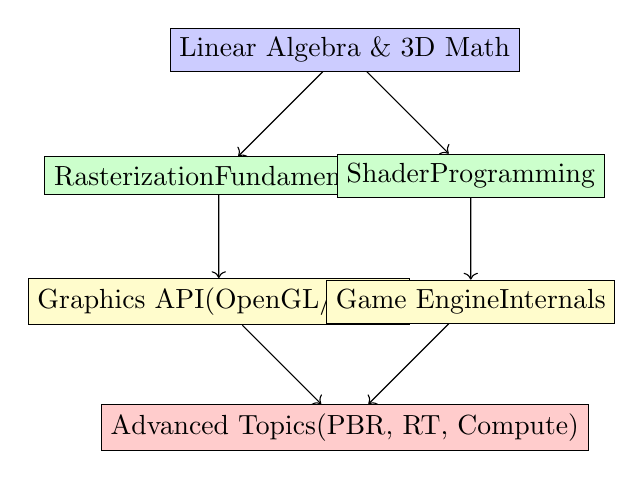
\begin{tikzpicture}[scale=0.8]
    % Learning path flowchart
    \node[draw, rectangle, fill=blue!20] (basics) at (0,4) {Linear Algebra \& 3D Math};
    
    \node[draw, rectangle, fill=green!20] (raster) at (-2,2) {Rasterization \\ Fundamentals};
    \node[draw, rectangle, fill=green!20] (shaders) at (2,2) {Shader \\ Programming};
    
    \node[draw, rectangle, fill=yellow!20] (api) at (-2,0) {Graphics API \\ (OpenGL/D3D)};
    \node[draw, rectangle, fill=yellow!20] (engine) at (2,0) {Game Engine \\ Internals};
    
    \node[draw, rectangle, fill=red!20] (advanced) at (0,-2) {Advanced Topics \\ (PBR, RT, Compute)};
    
    \draw[->] (basics) -- (raster);
    \draw[->] (basics) -- (shaders);
    \draw[->] (raster) -- (api);
    \draw[->] (shaders) -- (engine);
    \draw[->] (api) -- (advanced);
    \draw[->] (engine) -- (advanced);
\end{tikzpicture}
\end{center}

\begin{conceptbox}{Practice Projects}
\begin{enumerate}
    \item Software rasterizer implementation
    \item Simple OpenGL/Vulkan renderer
    \item Deferred rendering pipeline
    \item Shadow mapping techniques
    \item Post-processing effects
\end{enumerate}
\end{conceptbox}

\end{frame}


\end{document}
\endinput

% --- Section 6: From Casting to Tracing ---
\section{From Ray Casting to Ray Tracing}

\begin{frame}{Ray Casting vs Ray Tracing}
    \begin{center}
        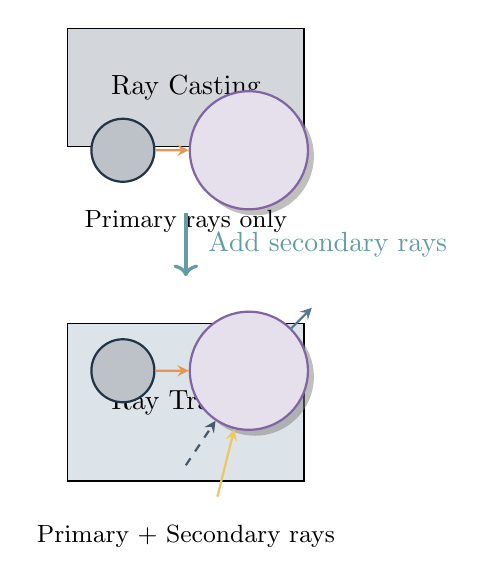
\begin{tikzpicture}[scale=0.8]
            % Ray Casting
            \node[rectangle, draw, minimum width=3cm, minimum height=1.5cm, fill=PrimaryColor!20] at (0,2) {Ray Casting};
            \node[eye] (eye1) at (-1,1) {};
            \node[sphere] (obj1) at (1,1) {};
            \draw[ray] (eye1) -- (obj1);
            \node[below] at (0,0.2) {\small Primary rays only};

            % Arrow
            \draw[->, very thick, AccentColor] (0,0) -- (0,-1);
            \node[right] at (0.2,-0.5) {\textcolor{AccentColor}{Add secondary rays}};

            % Ray Tracing
            \node[rectangle, draw, minimum width=3cm, minimum height=2cm, fill=SecondaryColor!20] at (0,-3) {Ray Tracing};
            \node[eye] (eye2) at (-1,-2.5) {};
            \node[sphere] (obj2) at (1,-2.5) {};
            \draw[ray] (eye2) -- (obj2);
            \draw[reflectray] (obj2) -- (2,-1.5);
            \draw[shadowray] (0,-4) -- (obj2);
            \draw[lightray] (0.5,-4.5) -- (obj2);
            \node[below] at (0,-4.8) {\small Primary + Secondary rays};
        \end{tikzpicture}
    \end{center}

    \begin{columns}
        \begin{column}{0.5\textwidth}
            \begin{raybox}{Ray Casting}
                \begin{itemize}
                    \item Eye rays only
                    \item Direct illumination
                    \item Fast but limited
                    \item Good for basic scenes
                \end{itemize}
            \end{raybox}
        \end{column}
        \begin{column}{0.5\textwidth}
            \begin{raybox}{Ray Tracing}
                \begin{itemize}
                    \item Multiple ray types
                    \item Global illumination
                    \item Slower but realistic
                    \item Reflections, shadows, refraction
                \end{itemize}
            \end{raybox}
        \end{column}
    \end{columns}
\end{frame}

\begin{frame}{Secondary Rays: The Magic Ingredients}
    \begin{center}
        \begin{tikzpicture}[scale=0.9]
            % Main scene setup
            \node[eye] (eye) at (0,0) {\faIcon{eye}};
            \node[sphere] (sphere) at (4,0) {};
            \node[circle, fill=LightColor, minimum size=0.8cm] (light) at (2,3) {\faIcon{lightbulb}};
            \node[sphere] (mirror) at (6,2) {};

            % Primary ray
            \draw[ray, very thick] (eye) -- (sphere);
            \node[below] at (2,-0.3) {\raycolor{1. Primary Ray}};

            % Shadow ray
            \draw[shadowray] (sphere) -- (light);
            \node[right] at (3.5,1.8) {\textcolor{DarkGray}{2. Shadow Ray}};

            % Reflection ray
            \draw[reflectray] (sphere) -- (mirror);
            \node[above] at (5,1.2) {\textcolor{SecondaryColor}{3. Reflection Ray}};

            % Ground plane
            \draw[thick, ObjectColor] (-1,-1.5) -- (7,-1.5);
            \draw[refractray] (sphere) -- (4,-1.5);
            \node[right] at (4.2,-1) {\textcolor{AccentColor}{4. Refraction Ray}};

            % Labels
            \node[above] at (2,3.5) {\textcolor{LightColor}{Light Source}};
            \node[above] at (6,2.8) {\textcolor{ObjectColor}{Mirror}};
            \node[below] at (4,-0.8) {\textcolor{ObjectColor}{Main Object}};
        \end{tikzpicture}
    \end{center}
\end{frame}

\begin{frame}{Recursive Ray Tracing}
    \begin{center}
        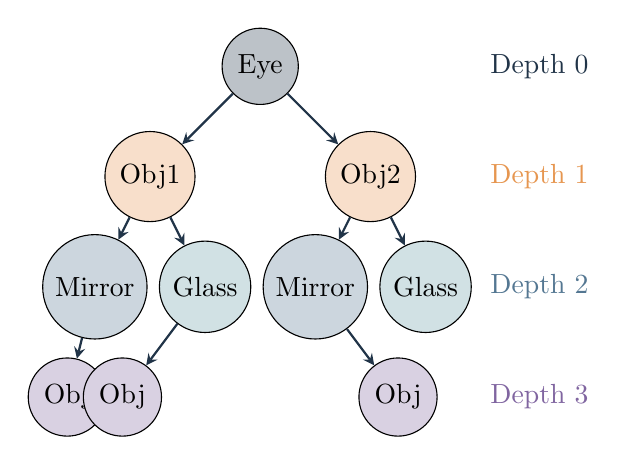
\begin{tikzpicture}[scale=0.7]
            % Tree structure showing recursion
            \node[circle, draw, fill=PrimaryColor!30] (root) at (0,4) {Eye};

            % Level 1
            \node[circle, draw, fill=RayColor!30] (obj1) at (-2,2) {Obj1};
            \node[circle, draw, fill=RayColor!30] (obj2) at (2,2) {Obj2};

            % Level 2
            \node[circle, draw, fill=SecondaryColor!30] (mirror1) at (-3,0) {Mirror};
            \node[circle, draw, fill=AccentColor!30] (glass1) at (-1,0) {Glass};
            \node[circle, draw, fill=SecondaryColor!30] (mirror2) at (1,0) {Mirror};
            \node[circle, draw, fill=AccentColor!30] (glass2) at (3,0) {Glass};

            % Level 3
            \node[circle, draw, fill=ObjectColor!30] (final1) at (-3.5,-2) {Obj};
            \node[circle, draw, fill=ObjectColor!30] (final2) at (-2.5,-2) {Obj};
            \node[circle, draw, fill=ObjectColor!30] (final3) at (2.5,-2) {Obj};

            % Connections
            \draw[arrow] (root) -- (obj1);
            \draw[arrow] (root) -- (obj2);
            \draw[arrow] (obj1) -- (mirror1);
            \draw[arrow] (obj1) -- (glass1);
            \draw[arrow] (obj2) -- (mirror2);
            \draw[arrow] (obj2) -- (glass2);
            \draw[arrow] (mirror1) -- (final1);
            \draw[arrow] (glass1) -- (final2);
            \draw[arrow] (mirror2) -- (final3);

            % Depth labels
            \node[right] at (4,4) {\textcolor{PrimaryColor}{Depth 0}};
            \node[right] at (4,2) {\textcolor{RayColor}{Depth 1}};
            \node[right] at (4,0) {\textcolor{SecondaryColor}{Depth 2}};
            \node[right] at (4,-2) {\textcolor{ObjectColor}{Depth 3}};
        \end{tikzpicture}
    \end{center}

    \begin{conceptbox}{Recursion Control}
        \textbf{Base Cases:} Maximum depth reached OR ray contribution becomes negligible
    \end{conceptbox}
\end{frame}

% --- Section 7: Advanced Topics ---
\section{Advanced Ray Tracing Effects}

\begin{frame}{Mirror Reflections}
    \begin{columns}
        \begin{column}{0.5\textwidth}
            \begin{mathbox}{Reflection Law}
                Given incident ray $\mathbf{d}$ and surface normal $\mathbf{n}$:
                \begin{align}
                    \mathbf{r} & = \mathbf{d} - 2(\mathbf{d} \cdot \mathbf{n})\mathbf{n}
                \end{align}

                \vspace{0.5cm}
                \textbf{Physical principle:}\\
                Angle of incidence = Angle of reflection
            \end{mathbox}
        \end{column}
        \begin{column}{0.5\textwidth}
            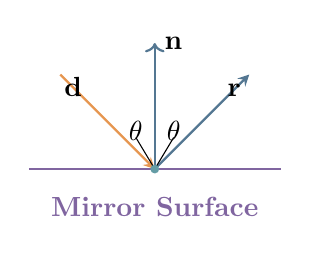
\begin{tikzpicture}[scale=0.8]
                % Mirror surface
                \draw[thick, ObjectColor] (-0.5,0) -- (3.5,0);
                \node[below] at (1.5,-0.3) {\objectcolor{Mirror Surface}};

                % Normal vector
                \draw[->, thick, SecondaryColor] (1.5,0) -- (1.5,2);
                \node[right] at (1.5,2) {$\mathbf{n}$};

                % Incident ray
                \draw[ray] (0,1.5) -- (1.5,0);
                \node[above left] at (0.5,1) {$\mathbf{d}$};

                % Reflected ray
                \draw[reflectray] (1.5,0) -- (3,1.5);
                \node[above right] at (2.5,1) {$\mathbf{r}$};

                % Angle indicators
                \draw[thin] (1.5,0) -- (1.2,0.5);
                \draw[thin] (1.5,0) -- (1.8,0.5);
                \node[above] at (1.2,0.3) {$\theta$};
                \node[above] at (1.8,0.3) {$\theta$};

                % Intersection point
                \fill[AccentColor] (1.5,0) circle (2pt);
            \end{tikzpicture}
        \end{column}
    \end{columns}

    \begin{center}
        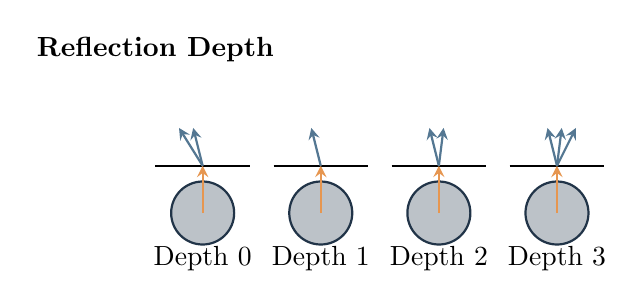
\begin{tikzpicture}[scale=0.6]
            % Depth progression
            \node[above] at (0,2) {\textbf{Reflection Depth}};

            \foreach \depth/\x in {0/0, 1/2.5, 2/5, 3/7.5} {
                    \begin{scope}[xshift=\x cm]
                        \draw[thick] (0,0) -- (2,0);
                        \node[eye] at (1,-1) {};
                        \draw[ray] (1,-1) -- (1,0);
                        \foreach \i in {1,...,\depth} {
                                \draw[reflectray] (1,0) -- (0.5+\i*0.3,0.8);
                            }
                        \node[below] at (1,-1.5) {Depth \depth};
                    \end{scope}
                }
        \end{tikzpicture}
    \end{center}
\end{frame}

\begin{frame}{Refraction and Snell's Law}
    \begin{columns}
        \begin{column}{0.5\textwidth}
            \begin{mathbox}{Snell's Law}
                \begin{align}
                    n_1 \sin\theta_1 & = n_2 \sin\theta_2
                \end{align}

                where:
                \begin{itemize}
                    \item $n_1, n_2$ = refractive indices
                    \item $\theta_1$ = incident angle
                    \item $\theta_2$ = refracted angle
                \end{itemize}

                \vspace{0.3cm}
                \textbf{Examples:}
                \begin{itemize}
                    \item Air: $n = 1.0$
                    \item Water: $n = 1.33$
                    \item Glass: $n = 1.5$
                \end{itemize}
            \end{mathbox}
        \end{column}
        \begin{column}{0.5\textwidth}
            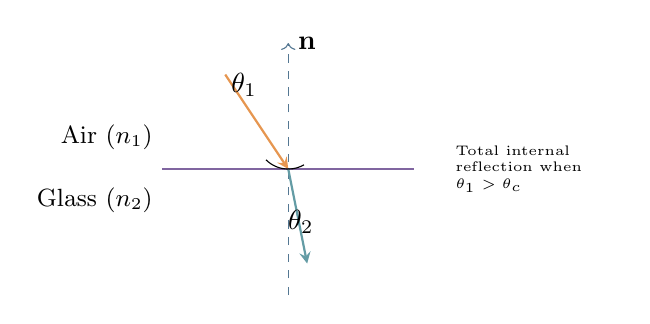
\begin{tikzpicture}[scale=0.8]
                % Interface
                \draw[thick, ObjectColor] (-1,0) -- (3,0);
                \node[left] at (-1,0.5) {\small Air ($n_1$)};
                \node[left] at (-1,-0.5) {\small Glass ($n_2$)};

                % Normal
                \draw[->, SecondaryColor, dashed] (1,-2) -- (1,2);
                \node[right] at (1,2) {$\mathbf{n}$};

                % Incident ray
                \draw[ray] (0,1.5) -- (1,0);
                \node[above] at (0.3,1) {$\theta_1$};

                % Refracted ray
                \draw[refractray] (1,0) -- (1.3,-1.5);
                \node[below] at (1.2,-0.5) {$\theta_2$};

                % Angles
                \draw[thin] (1,0) arc (270:225:0.5);
                \draw[thin] (1,0) arc (270:300:0.5);

                % Critical angle illustration
                \node[right] at (3.5,0) {
                    \begin{minipage}{2cm}
                        \tiny
                        Total internal\\
                        reflection when\\
                        $\theta_1 > \theta_c$
                    \end{minipage}
                };
            \end{tikzpicture}
        \end{column}
    \end{columns}

    \begin{conceptbox}{Physical Intuition}
        Light bends when moving between materials with different densities
    \end{conceptbox}
\end{frame}

\begin{frame}{Shadows: The Absence of Light}
    \begin{center}
        \begin{tikzpicture}[scale=0.9]
            % Light source
            \node[circle, fill=LightColor, minimum size=1cm] (light) at (0,3) {\faIcon{sun}};
            \node[above] at (0,3.8) {\textcolor{LightColor}{Light Source}};

            % Occluding object
            \node[sphere] (occluder) at (2,2) {};
            \node[above] at (2,2.8) {\textcolor{ObjectColor}{Occluder}};

            % Target object
            \node[sphere] (target) at (5,0) {};
            \node[below] at (5,-0.8) {\textcolor{ObjectColor}{Target}};

            % Eye
            \node[eye] (eye) at (7,0) {\faIcon{eye}};

            % Primary ray from eye
            \draw[ray] (eye) -- (target);
            \node[above] at (6,0.2) {\raycolor{Primary}};

            % Shadow ray (blocked)
            \draw[shadowray] (target) -- (occluder);
            \draw[shadowray, dashed] (occluder) -- (light);
            \node[left] at (3.5,1.2) {\textcolor{DarkGray}{Shadow Ray}};
            \node[right] at (3.5,1.5) {\textcolor{AccentColor}{BLOCKED!}};

            % Shadow region
            \fill[pattern=north east lines, pattern color=gray] (2.5,1.5) -- (4,0.5) -- (6,-0.5) -- (5.5,0.5) -- cycle;
            \node[right] at (6,0.8) {\textcolor{DarkGray}{Shadow}};
        \end{tikzpicture}
    \end{center}

    \begin{raybox}{Shadow Ray Algorithm}
        \textbf{For each intersection point:}
        \begin{enumerate}
            \item Cast ray toward each light source
            \item Check if ray intersects any object before reaching light
            \item If blocked → point is in shadow
            \item If clear → point is illuminated
        \end{enumerate}
    \end{raybox}
\end{frame}

% --- Section 8: Implementation Challenges ---
\section{Implementation Challenges}

\begin{frame}{The Floating Point Precision Problem}
    \begin{center}
        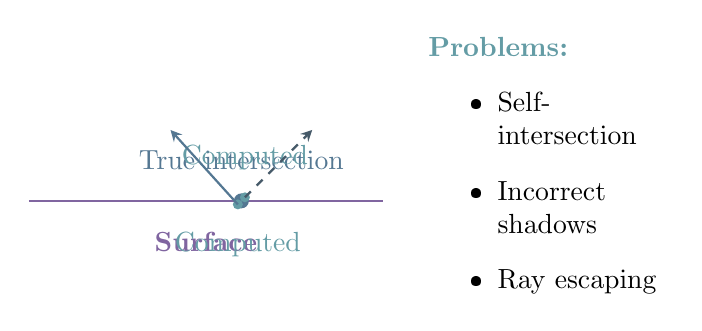
\begin{tikzpicture}[scale=0.9]
            % Surface
            \draw[thick, ObjectColor] (-1,0) -- (4,0);
            \node[below] at (1.5,-0.3) {\objectcolor{Surface}};

            % True intersection point
            \fill[SecondaryColor] (2,0) circle (3pt);
            \node[above] at (2,0.3) {\textcolor{SecondaryColor}{True intersection}};

            % Computed intersection points (with error)
            \fill[AccentColor] (1.95,-0.05) circle (2pt);
            \fill[AccentColor] (2.05,0.05) circle (2pt);
            \node[below] at (1.95,-0.3) {\textcolor{AccentColor}{Computed}};
            \node[above] at (2.05,0.3) {\textcolor{AccentColor}{Computed}};

            % Secondary rays from computed points
            \draw[reflectray] (1.95,-0.05) -- (1,1);
            \draw[shadowray] (2.05,0.05) -- (3,1);

            % Problems
            \node[right] at (4.5,0.5) {
                \begin{minipage}{3cm}
                    \textcolor{AccentColor}{\textbf{Problems:}}
                    \begin{itemize}
                        \item Self-intersection
                        \item Incorrect shadows
                        \item Ray escaping
                    \end{itemize}
                \end{minipage}
            };
        \end{tikzpicture}
    \end{center}

    \begin{conceptbox}{The Evil Epsilon}
        \textbf{Solution:} Add small offset $\varepsilon$ when starting secondary rays from surfaces\\
        \textbf{Challenge:} Too small → still problems; Too large → visible artifacts
    \end{conceptbox}
\end{frame}

\begin{frame}{Performance Considerations}
    \begin{columns}
        \begin{column}{0.5\textwidth}
            \begin{raybox}{Computational Complexity}
                \textbf{Basic ray tracing:}
                \begin{itemize}
                    \item $O(n \times m)$ where:
                    \item $n$ = number of pixels
                    \item $m$ = number of objects
                \end{itemize}

                \vspace{0.3cm}
                \textbf{With secondary rays:}
                \begin{itemize}
                    \item Exponential growth with depth
                    \item Multiple rays per intersection
                \end{itemize}
            \end{raybox}
        \end{column}
        \begin{column}{0.5\textwidth}
            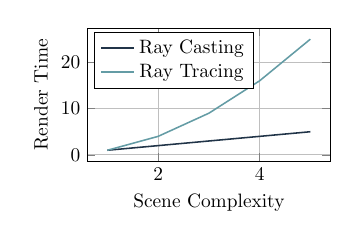
\begin{tikzpicture}[scale=0.7]
                % Performance graph
                \begin{axis}[
                        width=6cm,
                        height=4cm,
                        xlabel={Scene Complexity},
                        ylabel={Render Time},
                        grid=major,
                        legend pos=north west
                    ]
                    \addplot[thick, PrimaryColor] coordinates {(1,1) (2,2) (3,3) (4,4) (5,5)};
                    \addplot[thick, AccentColor] coordinates {(1,1) (2,4) (3,9) (4,16) (5,25)};
                    \legend{Ray Casting, Ray Tracing}
                \end{axis}
            \end{tikzpicture}

            \vspace{0.3cm}
            \textbf{Optimization strategies:}
            \begin{itemize}
                \item Spatial data structures
                \item Early ray termination
                \item Parallel processing
            \end{itemize}
        \end{column}
    \end{columns}
\end{frame}

% --- Section 9: Acceleration Structures ---
\section{Acceleration Structures: Making Ray Tracing Fast}

\begin{frame}{The Naive Approach Problem}
    \begin{center}
        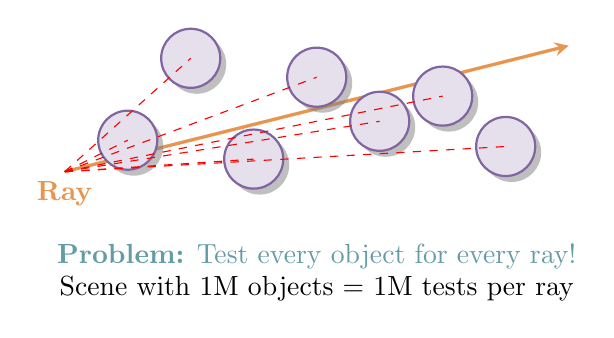
\begin{tikzpicture}[scale=0.8]
            % Ray
            \draw[ray, very thick] (0,0) -- (8,2);
            \node[below] at (0,0) {\raycolor{Ray}};

            % Many objects scattered
            \foreach \x/\y in {1/0.5, 2/1.8, 3/0.2, 4/1.5, 5/0.8, 6/1.2, 7/0.4} {
                    \node[sphere, scale=0.5] at (\x,\y) {};
                }

            % Intersection tests
            \foreach \x/\y in {1/0.5, 2/1.8, 3/0.2, 4/1.5, 5/0.8, 6/1.2, 7/0.4} {
                    \draw[dashed, red, thin] (0,0) -- (\x,\y);
                }

            \node[below] at (4,-1) {\textcolor{AccentColor}{\textbf{Problem:} Test every object for every ray!}};
            \node[below] at (4,-1.5) {Scene with 1M objects = 1M tests per ray};
        \end{tikzpicture}
    \end{center}

    \begin{conceptbox}{Computational Explosion}
        \textbf{Complexity:} For $N$ objects and $R$ rays → $O(N \times R)$ intersection tests\\
        \textbf{Real scenes:} Millions of triangles, millions of rays → Billions of tests!
    \end{conceptbox}
\end{frame}

\begin{frame}{Bounding Volume Hierarchy (BVH)}
    \begin{columns}
        \begin{column}{0.5\textwidth}
            \begin{raybox}{The Big Idea}
                \textbf{Divide and Conquer:}
                \begin{enumerate}
                    \item Group objects into bounding boxes
                    \item Build hierarchical tree structure
                    \item Test ray against boxes first
                    \item Only test objects in hit boxes
                \end{enumerate}
            \end{raybox}

            \vspace{0.3cm}
            \textbf{Key Benefits:}
            \begin{itemize}
                \item $O(\log N)$ instead of $O(N)$
                \item Massive speedup for complex scenes
                \item Works with any primitive type
            \end{itemize}
        \end{column}
        \begin{column}{0.5\textwidth}
            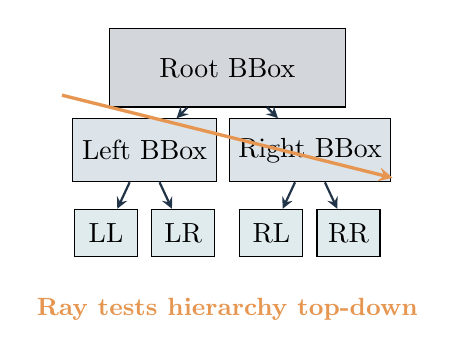
\begin{tikzpicture}[scale=0.7]
                % BVH Tree structure
                \node[rectangle, draw, fill=PrimaryColor!20, minimum width=3cm, minimum height=1cm] (root) at (0,3) {Root BBox};

                \node[rectangle, draw, fill=SecondaryColor!20, minimum width=1.3cm, minimum height=0.8cm] (left) at (-1.5,1.5) {Left BBox};
                \node[rectangle, draw, fill=SecondaryColor!20, minimum width=1.3cm, minimum height=0.8cm] (right) at (1.5,1.5) {Right BBox};

                \node[rectangle, draw, fill=AccentColor!20, minimum width=0.8cm, minimum height=0.6cm] (ll) at (-2.2,0) {LL};
                \node[rectangle, draw, fill=AccentColor!20, minimum width=0.8cm, minimum height=0.6cm] (lr) at (-0.8,0) {LR};
                \node[rectangle, draw, fill=AccentColor!20, minimum width=0.8cm, minimum height=0.6cm] (rl) at (0.8,0) {RL};
                \node[rectangle, draw, fill=AccentColor!20, minimum width=0.8cm, minimum height=0.6cm] (rr) at (2.2,0) {RR};

                % Tree connections
                \draw[arrow] (root) -- (left);
                \draw[arrow] (root) -- (right);
                \draw[arrow] (left) -- (ll);
                \draw[arrow] (left) -- (lr);
                \draw[arrow] (right) -- (rl);
                \draw[arrow] (right) -- (rr);

                % Ray traversal
                \draw[ray, very thick] (-3,2.5) -- (3,1);
                \node[below] at (0,-1) {\small \raycolor{Ray tests hierarchy top-down}};
            \end{tikzpicture}
        \end{column}
    \end{columns}
\end{frame}

\begin{frame}{BVH Construction and Traversal}
    \begin{columns}
        \begin{column}{0.5\textwidth}
            \begin{mathbox}{Construction Algorithm}
                \textbf{Recursive subdivision:}
                \begin{enumerate}
                    \item Compute bounding box for all objects
                    \item Choose split axis (longest dimension)
                    \item Sort objects by centroid
                    \item Split into two groups
                    \item Recursively build subtrees
                \end{enumerate}

                \vspace{0.3cm}
                \textbf{Split strategies:}
                \begin{itemize}
                    \item Median split
                    \item Surface Area Heuristic (SAH)
                    \item Spatial splits
                \end{itemize}
            \end{mathbox}
        \end{column}
        \begin{column}{0.5\textwidth}
            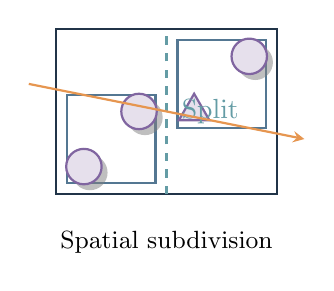
\begin{tikzpicture}[scale=0.7]
                % Scene with objects and bounding boxes
                \draw[thick, PrimaryColor] (-0.5,-0.5) rectangle (3.5,2.5);
                \draw[thick, SecondaryColor] (-0.3,-0.3) rectangle (1.3,1.3);
                \draw[thick, SecondaryColor] (1.7,0.7) rectangle (3.3,2.3);

                % Objects
                \node[sphere, scale=0.3] at (0,0) {};
                \node[sphere, scale=0.3] at (1,1) {};
                \node[triangle, scale=0.3] at (2,1) {};
                \node[sphere, scale=0.3] at (3,2) {};

                % Split line
                \draw[dashed, AccentColor, thick] (1.5,-0.5) -- (1.5,2.5);
                \node[right] at (1.6,1) {\textcolor{AccentColor}{Split}};

                % Ray traversal example
                \draw[ray] (-1,1.5) -- (4,0.5);

                \node[below] at (1.5,-1) {\small Spatial subdivision};
            \end{tikzpicture}

            \vspace{0.3cm}
            \begin{conceptbox}{Traversal}
                \textbf{Stack-based traversal:} Test bounding boxes, push hit children onto stack
            \end{conceptbox}
        \end{column}
    \end{columns}
\end{frame}

% --- Section 10: Hardware Acceleration ---
\section{Hardware Ray Tracing Revolution}

\begin{frame}{The Hardware Revolution}
    \begin{center}
        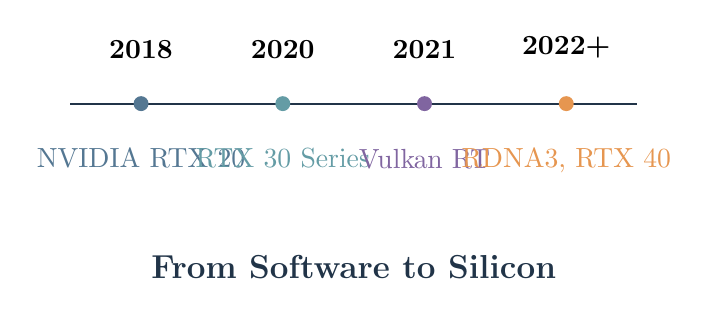
\begin{tikzpicture}[scale=0.9]
            % Timeline
            \draw[thick, PrimaryColor] (0,0) -- (8,0);

            % Milestones
            \node[above] at (1,0.5) {\textbf{2018}};
            \node[below] at (1,-0.5) {\textcolor{SecondaryColor}{NVIDIA RTX 20}};
            \fill[SecondaryColor] (1,0) circle (3pt);

            \node[above] at (3,0.5) {\textbf{2020}};
            \node[below] at (3,-0.5) {\textcolor{AccentColor}{RTX 30 Series}};
            \fill[AccentColor] (3,0) circle (3pt);

            \node[above] at (5,0.5) {\textbf{2021}};
            \node[below] at (5,-0.5) {\textcolor{ObjectColor}{Vulkan RT}};
            \fill[ObjectColor] (5,0) circle (3pt);

            \node[above] at (7,0.5) {\textbf{2022+}};
            \node[below] at (7,-0.5) {\textcolor{RayColor}{RDNA3, RTX 40}};
            \fill[RayColor] (7,0) circle (3pt);

            \node[below] at (4,-2) {\large \textcolor{PrimaryColor}{\textbf{From Software to Silicon}}};
        \end{tikzpicture}
    \end{center}

    \begin{columns}
        \begin{column}{0.5\textwidth}
            \textbf{Hardware Features:}
            \begin{itemize}
                \item Dedicated RT cores
                \item Hardware BVH traversal
                \item Triangle intersection units
                \item Tensor cores for denoising
            \end{itemize}
        \end{column}
        \begin{column}{0.5\textwidth}
            \textbf{Performance Impact:}
            \begin{itemize}
                \item 10-100x speedup over compute shaders
                \item Real-time ray tracing in games
                \item Interactive path tracing
                \item AI-accelerated denoising
            \end{itemize}
        \end{column}
    \end{columns}
\end{frame}

\begin{frame}{RTX Architecture Deep Dive}
    \begin{center}
        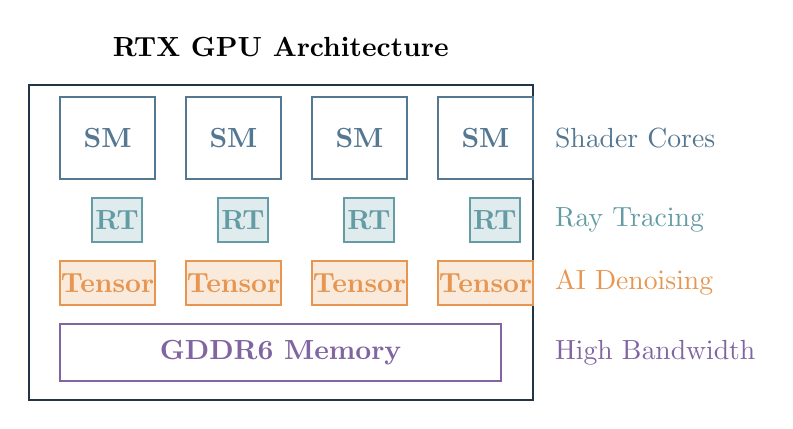
\begin{tikzpicture}[scale=0.8]
            % GPU die representation
            \draw[thick, PrimaryColor] (0,0) rectangle (8,5);
            \node[above] at (4,5.3) {\textbf{RTX GPU Architecture}};

            % Streaming Multiprocessors
            \foreach \x in {0.5,2.5,4.5,6.5} {
                    \draw[SecondaryColor, thick] (\x,3.5) rectangle (\x+1.5,4.8);
                    \node at (\x+0.75,4.15) {\textcolor{SecondaryColor}{\textbf{SM}}};
                }

            % RT Cores
            \foreach \x in {1,3,5,7} {
                    \draw[AccentColor, thick, fill=AccentColor!20] (\x,2.5) rectangle (\x+0.8,3.2);
                    \node at (\x+0.4,2.85) {\textcolor{AccentColor}{\textbf{RT}}};
                }

            % Tensor Cores
            \foreach \x in {0.5,2.5,4.5,6.5} {
                    \draw[RayColor, thick, fill=RayColor!20] (\x,1.5) rectangle (\x+1.5,2.2);
                    \node at (\x+0.75,1.85) {\textcolor{RayColor}{\textbf{Tensor}}};
                }

            % Memory
            \draw[ObjectColor, thick] (0.5,0.3) rectangle (7.5,1.2);
            \node at (4,0.75) {\textcolor{ObjectColor}{\textbf{GDDR6 Memory}}};

            % Labels
            \node[right] at (8.2,4.15) {\textcolor{SecondaryColor}{Shader Cores}};
            \node[right] at (8.2,2.85) {\textcolor{AccentColor}{Ray Tracing}};
            \node[right] at (8.2,1.85) {\textcolor{RayColor}{AI Denoising}};
            \node[right] at (8.2,0.75) {\textcolor{ObjectColor}{High Bandwidth}};
        \end{tikzpicture}
    \end{center}

    \begin{raybox}{RT Core Functions}
        \textbf{Hardware accelerated:} BVH traversal, ray-triangle intersection, ray-box intersection\\
        \textbf{Result:} Massive parallel ray processing with dedicated silicon
    \end{raybox}
\end{frame}

\begin{frame}{Modern Ray Tracing APIs}
    \begin{columns}
        \begin{column}{0.5\textwidth}
            \begin{conceptbox}{DirectX Raytracing (DXR)}
                \textbf{Microsoft's API:}
                \begin{itemize}
                    \item Raytracing Pipeline State Objects
                    \item Acceleration Structure builds
                    \item Ray generation/intersection/hit shaders
                    \item Widely adopted in games
                \end{itemize}
            \end{conceptbox}

            \vspace{0.3cm}
            \begin{conceptbox}{Vulkan Ray Tracing}
                \textbf{Cross-platform standard:}
                \begin{itemize}
                    \item VK\_KHR\_ray\_tracing\_pipeline
                    \item Lower-level control
                    \item Multi-vendor support
                    \item Mobile and desktop
                \end{itemize}
            \end{conceptbox}
        \end{column}
        \begin{column}{0.5\textwidth}
            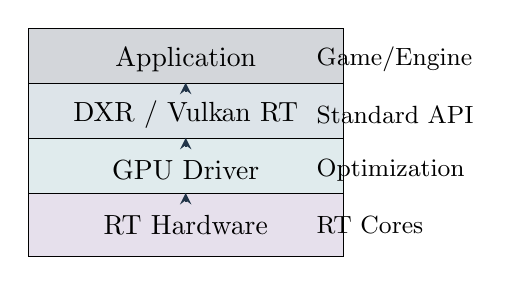
\begin{tikzpicture}[scale=0.7]
                % API stack
                \node[rectangle, draw, fill=PrimaryColor!20, minimum width=4cm, minimum height=0.8cm] (app) at (0,3) {Application};
                \node[rectangle, draw, fill=SecondaryColor!20, minimum width=4cm, minimum height=0.8cm] (api) at (0,2) {DXR / Vulkan RT};
                \node[rectangle, draw, fill=AccentColor!20, minimum width=4cm, minimum height=0.8cm] (driver) at (0,1) {GPU Driver};
                \node[rectangle, draw, fill=ObjectColor!20, minimum width=4cm, minimum height=0.8cm] (hw) at (0,0) {RT Hardware};

                % Arrows
                \draw[arrow] (app) -- (api);
                \draw[arrow] (api) -- (driver);
                \draw[arrow] (driver) -- (hw);

                % Side annotations
                \node[right] at (2.2,3) {\small Game/Engine};
                \node[right] at (2.2,2) {\small Standard API};
                \node[right] at (2.2,1) {\small Optimization};
                \node[right] at (2.2,0) {\small RT Cores};
            \end{tikzpicture}

            \vspace{0.5cm}
            \textbf{Key Innovation:}
            \begin{itemize}
                \item Shader-driven ray tracing
                \item Flexible hit/miss handling
                \item Integration with rasterization
                \item Real-time performance
            \end{itemize}
        \end{column}
    \end{columns}
\end{frame}

% --- Section 11: Path Tracing ---
\section{Path Tracing: The Ultimate Goal}

\begin{frame}{Beyond Ray Tracing: Path Tracing}
    \begin{center}
        \begin{tikzpicture}[scale=0.8]
            % Scene setup
            \node[circle, fill=LightColor, minimum size=1cm] (light) at (1,4) {\faIcon{sun}};
            \node[sphere] (sphere1) at (3,2) {};
            \node[sphere] (sphere2) at (5,1) {};
            \node[eye] (eye) at (7,2) {\faIcon{eye}};

            % Multiple path samples
            \draw[ray, bend left=10] (eye) to (sphere2);
            \draw[reflectray, bend right=15] (sphere2) to (sphere1);
            \draw[lightray, bend left=20] (sphere1) to (light);

            \draw[ray, bend left=20] (eye) to (sphere2);
            \draw[reflectray, bend left=10] (sphere2) to (3,4);
            \draw[lightray] (3,4) to (light);

            \draw[ray, bend right=10] (eye) to (sphere2);
            \draw[reflectray, bend right=25] (sphere2) to (sphere1);
            \draw[refractray, bend left=15] (sphere1) to (2,0);

            % Path labels
            \node[below] at (4,-0.5) {\raycolor{\textbf{Multiple Random Paths}}};
            \node[above] at (4,4.8) {\textcolor{LightColor}{\textbf{Monte Carlo Integration}}};
        \end{tikzpicture}
    \end{center}

    \begin{columns}
        \begin{column}{0.5\textwidth}
            \begin{raybox}{Ray Tracing Limitations}
                \begin{itemize}
                    \item Perfect mirrors only
                    \item Direct illumination focus
                    \item Limited global effects
                    \item Deterministic sampling
                \end{itemize}
            \end{raybox}
        \end{column}
        \begin{column}{0.5\textwidth}
            \begin{raybox}{Path Tracing Advantages}
                \begin{itemize}
                    \item Physically accurate lighting
                    \item Global illumination
                    \item Soft shadows, caustics
                    \item Unbiased rendering
                \end{itemize}
            \end{raybox}
        \end{column}
    \end{columns}
\end{frame}

\begin{frame}{The Rendering Equation}
    \begin{center}
        \begin{mathbox}{The Holy Grail of Computer Graphics}
            \begin{align}
                L_o(\mathbf{p}, \omega_o) = L_e(\mathbf{p}, \omega_o) + \int_\Omega f(\mathbf{p}, \omega_i, \omega_o) L_i(\mathbf{p}, \omega_i) (\mathbf{n} \cdot \omega_i) d\omega_i
            \end{align}
        \end{mathbox}
    \end{center}

    \begin{columns}
        \begin{column}{0.5\textwidth}
            \textbf{Components:}
            \begin{itemize}
                \item $L_o$ = Outgoing radiance
                \item $L_e$ = Emitted light
                \item $f$ = BRDF (material properties)
                \item $L_i$ = Incoming radiance
                \item $\Omega$ = Hemisphere of directions
            \end{itemize}
        \end{column}
        \begin{column}{0.5\textwidth}
            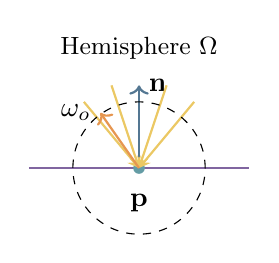
\begin{tikzpicture}[scale=0.7]
                % Surface point
                \draw[thick, ObjectColor] (-1,0) -- (3,0);
                \fill[AccentColor] (1,0) circle (3pt);
                \node[below] at (1,-0.3) {$\mathbf{p}$};

                % Normal
                \draw[->, SecondaryColor, thick] (1,0) -- (1,1.5);
                \node[right] at (1,1.5) {$\mathbf{n}$};

                % Incoming light hemisphere
                \draw[lightray] (0,1.2) -- (1,0);
                \draw[lightray] (0.5,1.5) -- (1,0);
                \draw[lightray] (1.5,1.5) -- (1,0);
                \draw[lightray] (2,1.2) -- (1,0);

                % Outgoing direction
                \draw[->, RayColor, thick] (1,0) -- (0.3,1);
                \node[left] at (0.3,1) {$\omega_o$};

                % Hemisphere
                \draw[dashed] (1,0) circle (1.2);
                \node[above] at (1,1.8) {\small Hemisphere $\Omega$};
            \end{tikzpicture}
        \end{column}
    \end{columns}

    \begin{conceptbox}{The Challenge}
        \textbf{Integral:} Infinite directions to sample → Monte Carlo approximation needed
    \end{conceptbox}
\end{frame}

\begin{frame}{Path Tracing vs Ray Tracing}
    \begin{center}
        \begin{tikzpicture}[scale=0.7]
            % Ray Tracing side
            \node[above] at (-2,3) {\textbf{Ray Tracing}};
            \node[eye] (eye1) at (-4,1) {};
            \node[triangle] (near1) at (-2,1.2) {};
            \node[triangle] (far1) at (-1,1) {};
            \draw[ray] (eye1) -- (-2,1.5) -- (-0.5,1.2);
            \draw[ray] (eye1) -- (-2,0.5) -- (-0.5,0.8);
            \node[below] at (-3,0.2) {\small Converging rays};
            \node[below] at (-3,-0.1) {\small Size $\propto$ 1/distance};

            % vs
            \node at (0,1) {\huge \textcolor{AccentColor}{vs}};

            % Path Tracing side
            \node[above] at (2,3) {\textbf{Path Tracing}};
            \node[eye] (eye2) at (0.5,1) {};
            \node[sphere] (obj2) at (2,1) {};
            \node[sphere] (obj3) at (3,2) {};
            \node[circle, fill=LightColor, minimum size=0.6cm] (light2) at (4,0.5) {};

            % Multiple random paths
            \draw[ray, bend left=10] (eye2) to (sphere2);
            \draw[reflectray, bend right=15] (sphere2) to (sphere1);
            \draw[lightray, bend left=20] (sphere1) to (light);

            \draw[ray, bend left=20] (eye2) to (sphere2);
            \draw[reflectray, bend left=10] (sphere2) to (3,4);
            \draw[lightray] (3,4) to (light);

            \draw[ray, bend right=10] (eye2) to (sphere2);
            \draw[reflectray, bend right=25] (sphere2) to (sphere1);
            \draw[refractray, bend left=15] (sphere1) to (2,0);

            % Path labels
            \node[below] at (4,-0.5) {\raycolor{\textbf{Multiple Random Paths}}};
            \node[above] at (4,4.8) {\textcolor{LightColor}{\textbf{Monte Carlo Integration}}};
        \end{tikzpicture}
    \end{center}

    \begin{columns}
        \begin{column}{0.5\textwidth}
            \begin{raybox}{Ray Tracing Limitations}
                \begin{itemize}
                    \item Perfect mirrors only
                    \item Direct illumination focus
                    \item Limited global effects
                    \item Deterministic sampling
                \end{itemize}
            \end{raybox}
        \end{column}
        \begin{column}{0.5\textwidth}
            \begin{raybox}{Path Tracing Advantages}
                \begin{itemize}
                    \item Physically accurate lighting
                    \item Global illumination
                    \item Soft shadows, caustics
                    \item Unbiased rendering
                \end{itemize}
            \end{raybox}
        \end{column}
    \end{columns}
\end{frame}

% --- Section 12: Shading Models Preview ---
\section{The Art of Shading (Preview)}

\begin{frame}{From Geometry to Beauty}
    \begin{center}
        \large \textcolor{PrimaryColor}{We've traced rays and found intersections...}\\
        \vspace{0.5cm}
        \huge \textcolor{AccentColor}{Now what color should that pixel be?}
    \end{center}

    \begin{columns}
        \begin{column}{0.5\textwidth}
            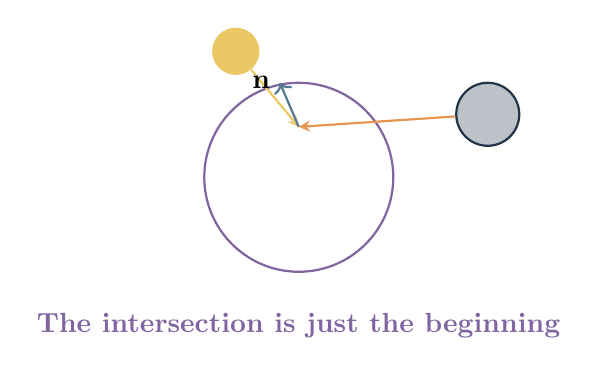
\begin{tikzpicture}[scale=0.8]
                % Simple sphere with different shading
                \draw[thick, ObjectColor] (0,0) circle (1.5);

                % Light direction
                \node[circle, fill=LightColor, minimum size=0.6cm] (light) at (-1,2) {};
                \draw[lightray] (light) -- (0,0.8);

                % Normal at surface
                \draw[->, SecondaryColor, thick] (0,0.8) -- (-0.3,1.5);
                \node[left] at (-0.3,1.5) {$\mathbf{n}$};

                % Eye direction
                \node[eye] (eye) at (3,1) {};
                \draw[ray] (eye) -- (0,0.8);

                \node[below] at (0,-2) {\textcolor{ObjectColor}{\textbf{The intersection is just the beginning}}};
            \end{tikzpicture}
        \end{column}
        \begin{column}{0.5\textwidth}
            \textbf{Shading determines:}
            \begin{itemize}
                \item Surface appearance
                \item Material properties
                \item Light interaction
                \item Visual realism
            \end{itemize}

            \vspace{0.5cm}
            \alert{Next lesson:} Deep dive into shading models!
        \end{column}
    \end{columns}
\end{frame}

\begin{frame}{Shading Models: A Sneak Peek}
    \begin{center}
        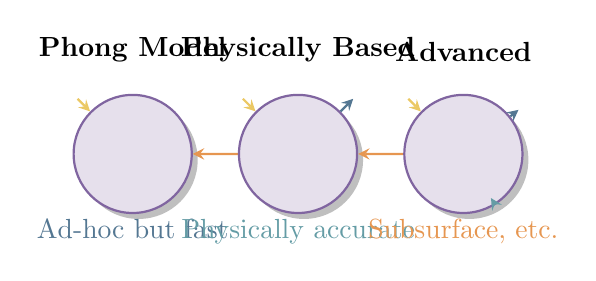
\begin{tikzpicture}[scale=0.7]
            % Phong model illustration
            \node[above] at (-3,2.5) {\textbf{Phong Model}};
            \node[sphere] (phong) at (-3,1) {};
            \draw[lightray] (-4,2) -- (phong);
            \draw[ray] (-1,1) -- (phong);
            \node[below] at (-3,0) {\textcolor{SecondaryColor}{Ad-hoc but fast}};

            % PBR illustration  
            \node[above] at (0,2.5) {\textbf{Physically Based}};
            \node[sphere] (pbr) at (0,1) {};
            \draw[lightray] (-1,2) -- (pbr);
            \draw[reflectray] (pbr) -- (1,2);
            \draw[ray] (2,1) -- (pbr);
            \node[below] at (0,0) {\textcolor{AccentColor}{Physically accurate}};

            % Advanced illustration
            \node[above] at (3,2.5) {\textbf{Advanced}};
            \node[sphere] (adv) at (3,1) {};
            \draw[lightray] (2,2) -- (adv);
            \draw[refractray] (adv) -- (3.5,0.2);
            \draw[reflectray] (adv) -- (4,1.8);
            \node[below] at (3,0) {\textcolor{RayColor}{Subsurface, etc.}};
        \end{tikzpicture}
    \end{center}

    \begin{columns}
        \begin{column}{0.33\textwidth}
            \begin{conceptbox}{Phong/Blinn-Phong}
                \textbf{Components:}
                \begin{itemize}
                    \item Ambient
                    \item Diffuse
                    \item Specular
                \end{itemize}
                \textbf{Pro:} Fast, simple\\
                \textbf{Con:} Not physically accurate
            \end{conceptbox}
        \end{column}
        \begin{column}{0.33\textwidth}
            \begin{conceptbox}{Physically Based}
                \textbf{Based on:}
                \begin{itemize}
                    \item Energy conservation
                    \item Fresnel equations
                    \item Microfacet theory
                \end{itemize}
                \textbf{Pro:} Realistic, consistent\\
                \textbf{Con:} More complex
            \end{conceptbox}
        \end{column}
        \begin{column}{0.33\textwidth}
            \begin{conceptbox}{Advanced Models}
                \textbf{Features:}
                \begin{itemize}
                    \item Subsurface scattering
                    \item Volumetric effects
                    \item Layered materials
                \end{itemize}
                \textbf{Pro:} Ultimate realism\\
                \textbf{Con:} Computationally expensive
            \end{conceptbox}
        \end{column}
    \end{columns}
\end{frame}

% --- Section 13: Applications and Future ---
\section{Applications and Future}

\begin{frame}{Ray Tracing in the Real World}
    \begin{center}
        \begin{tikzpicture}[scale=0.8]
            % Applications
            \node[rectangle, rounded corners, fill=PrimaryColor!20, minimum width=2.5cm, minimum height=1.5cm] (movies) at (0,2) {Movies \& VFX};
            \node[rectangle, rounded corners, fill=SecondaryColor!20, minimum width=2.5cm, minimum height=1.5cm] (games) at (4,2) {Video Games};
            \node[rectangle, rounded corners, fill=AccentColor!20, minimum width=2.5cm, minimum height=1.5cm] (arch) at (0,0) {Architecture};
            \node[rectangle, rounded corners, fill=ObjectColor!20, minimum width=2.5cm, minimum height=1.5cm] (product) at (4,0) {Product Design};

            % Center
            \node[circle, fill=LightColor, minimum size=2cm] (center) at (2,1) {\textbf{Ray Tracing}};

            % Connections
            \draw[arrow] (center) -- (movies);
            \draw[arrow] (center) -- (games);
            \draw[arrow] (center) -- (arch);
            \draw[arrow] (center) -- (product);

            % Icons
            \node at (0,2.5) {\faIcon{film}};
            \node at (4,2.5) {\faIcon{gamepad}};
            \node at (0,0.5) {\faIcon{building}};
            \node at (4,0.5) {\faIcon{car}};
        \end{tikzpicture}
    \end{center}

    \begin{columns}
        \begin{column}{0.5\textwidth}
            \textbf{Traditional (Offline):}
            \begin{itemize}
                \item Movie rendering
                \item Architectural visualization
                \item Product design
                \item Scientific simulation
            \end{itemize}
        \end{column}
        \begin{column}{0.5\textwidth}
            \textbf{Modern (Real-time):}
            \begin{itemize}
                \item RTX graphics cards
                \item Video games
                \item VR/AR applications
                \item Interactive design
            \end{itemize}
        \end{column}
    \end{columns}
\end{frame}

\begin{frame}{The Future is Bright}
    \begin{conceptbox}{Hardware Acceleration}
        \textbf{Modern GPUs:} Dedicated ray tracing cores, massive parallelization
    \end{conceptbox}

    \vspace{0.3cm}

    \begin{columns}
        \begin{column}{0.5\textwidth}
            \textbf{Emerging Techniques:}
            \begin{itemize}
                \item Machine learning denoising
                \item Hybrid rendering
                \item Path tracing
                \item Photon mapping
            \end{itemize}
        \end{column}
        \begin{column}{0.5\textwidth}
            \textbf{New Applications:}
            \begin{itemize}
                \item Medical imaging
                \item Autonomous vehicles
                \item Metaverse platforms
                \item Scientific visualization
            \end{itemize}
        \end{column}
    \end{columns}

    \vspace{0.5cm}

    \begin{center}
        \large \textcolor{PrimaryColor}{\textbf{Ray tracing is becoming the future of computer graphics!}}
    \end{center}
\end{frame}

% --- Conclusion ---
\section{Wrapping Up}

\begin{frame}{Key Takeaways}
    \begin{enumerate}
        \item \highlight{Ray tracing simulates light transport} by reversing the natural process
        \item \highlight{Mathematical foundation} involves solving intersection equations for different geometric primitives
        \item \highlight{Secondary rays} enable realistic effects like reflections, refractions, and shadows
        \item \highlight{Implementation challenges} include floating-point precision and performance optimization
        \item \highlight{Real-world impact} spans from Hollywood movies to real-time gaming
    \end{enumerate}

    \vspace{0.5cm}

    \begin{center}
        \begin{tikzpicture}[scale=0.6]
            % Final illustration
            \node[eye] (eye) at (0,0) {\faIcon{eye}};
            \node[sphere] at (2,0) {};
            \node[sphere] at (3,1) {};
            \node[triangle] at (4,-1) {};
            \node[circle, fill=LightColor, minimum size=0.8cm] at (2,2) {\faIcon{lightbulb}};

            \draw[ray] (eye) -- (2,0) -- (4,1);
            \draw[reflectray] (2,0) -- (3,1);
            \draw[shadowray] (2,0) -- (2,2);
            \draw[refractray] (2,0) -- (4,-1);

            \node[below] at (2,-2) {\textcolor{PrimaryColor}{\textbf{The art and science of light}}};
        \end{tikzpicture}
    \end{center}
\end{frame}
\end{document}